%%%%%%%%%%%%%%%%%%%%%%%%%%%%%%%%%%%%%%%%%%%%%%%%%%%%%%%%%%%%%%%%%%%%%%%%%%%%%%
\section{Decays of the SM Higgs boson}
\setcounter{equation}{0}
\renewcommand{\theequation}{2.\arabic{equation}}


In the Standard Model, once the Higgs mass is fixed, the profile of the
Higgs particle is uniquely determined. The Higgs couplings to gauge bosons 
and fermions are directly proportional to the masses of the particles and
the Higgs boson will have the tendency to decay into the heaviest ones 
allowed by phase space. Since the pole masses of the gauge bosons and 
fermions are known [the electron and light quark masses are too small to be
relevant]
\beq 
M_Z=91.187~{\rm GeV} \ , \ M_W=80.425~{\rm GeV} \ , \ m_\tau=1.777~{\rm GeV} 
\ , \  m_\mu= 0.106~{\rm GeV} \, , \non \\ 
m_t=178 \pm 4.3~{\rm GeV} \ , \
m_b=4.88 \pm 0.07~{\rm GeV} \ , \
m_c=1.64 \pm 0.07~{\rm GeV} \hspace*{1cm}
\label{allmasses}
\eeq
all the partial widths for the Higgs decays into these particles can be 
predicted.\s 

The decay widths into massive gauge bosons $V=W,Z$ are directly proportional 
to the $HVV$ couplings, which in the SM are given in terms of the fields by 
\begin{eqnarray}
{\cal L}(HVV)&=&\left(\sqrt2G_\mu\right)^{1/2}M_V^2HV^\mu V_\mu 
%\ \sim \ G_\mu^{1/2}HF^{\mu\nu}F_{\mu\nu}
\label{HVVcp}
\end{eqnarray}
These are S--wave couplings and even under parity and charge conjugation,
corresponding to the $J^{\rm PC}=0^{++}$ assignment of the Higgs  spin and
parity quantum numbers. The decay widths into fermions are proportional to
the $H f\bar{f}$ couplings which are of the scalar type
\beq
g_{H\bar{f}f} \propto \frac{m_f}{v} =  (\sqrt{2}G_\mu)^{1/2} m_f 
\label{Hffcp}
\eeq
In this section, we will discuss all the decay modes of the SM Higgs boson: 
decays into quarks and leptons, into real or virtual gauge bosons and loop 
induced decays into photons [including $Z\gamma$ final states] and gluons, and
summarize the important QCD and electroweak radiative corrections to 
these processes. \s 

The $J^{\rm PC}=0^{++}$ quantum numbers of the SM Higgs particle lead also to
unique predictions for the angular and energy distributions of the partial
decay widths.  Whenever possible, we will confront these properties with those
of an  hypothetical CP--odd Higgs particle\footnote{The decays of the Higgs
bosons \cite{Hdecay-Effective,Eff-decays,Eff-Romao} in the general case of anomalous Higgs couplings 
\cite{HVV-Effective,Hff-Effective} will be discussed in another part of this 
review.}, 
that we will denote by $A$, and  which is predicted in many extensions of the 
SM. In this case, the Higgs coupling to vector gauge bosons is a P--wave 
coupling corresponding to the $J^{\rm PC}=0^{+-}$ assignment and, if CP 
symmetry is conserved, does not occur at the tree--level and is only induced by 
higher loop effects.  With $\eta$ being a dimensionless factor, the effective 
point--like coupling can be written as 
\begin{eqnarray}
{\cal L}(AVV)= {1 \over 4} \eta \left(\sqrt2 G_\mu \right)^{1/2}M_V^2 A
V^{\mu\nu} \widetilde V_{\mu\nu} \ , \ \ \ \ \widetilde V^{\mu\nu}= 
\epsilon^{\mu\nu\rho
\sigma} V_{\rho\sigma}
\label{AVVcp}
\end{eqnarray}
In the presence of fermions, the couplings of the $A$ boson are of the 
pseudoscalar type
\beq
g_{A\bar{f}f} \propto \frac{m_f}{v} \gamma_5 =  (\sqrt{2}G_\mu)^{1/2} m_f 
\gamma_5
\label{Affcp}
\eeq

\subsection{Decays to quarks and leptons} 

\subsubsection{The Born approximation}

In the Born approximation, the partial width of the Higgs boson decay into
fermion pairs, Fig.~2.1, is given by \cite{HffBorn,EGN}
\beq
\Gamma_{\rm Born} (H \ra f \bar{f})= \frac{G_\mu N_c}{4 \sqrt{2} \pi} \,  
M_H \, 
m_f^2 \, 
\beta_f^3
\eeq
with $\beta=(1- 4m_f^2/M_H^2)^{1/2}$ being the velocity of the fermions in the 
final state and $N_c$ the color factor $N_c=3\, (1)$ for quarks (leptons). In
the lepton case, only decays into $\tau^+ \tau^-$ pairs and, to a much lesser 
extent, decays into muon pairs are relevant.

\vspace*{-8mm}
\begin{center}
\hspace*{6cm}
\begin{picture}(300,100)(0,0)
\SetWidth{1.}
\SetScale{1.2}
\DashLine(0,50)(40,50){4}
\ArrowLine(40,50)(70,75)
\ArrowLine(40,50)(70,25)
\Text(49,60)[]{{\blue{\large $\bullet$}}}
\Text(27,70)[]{\blue{$H$}}
\Text(90,80)[]{$f$}
\Text(90,40)[]{$\bar{f}$}
\end{picture}
\end{center}
\vspace*{-1.4cm}
\centerline{\it Figure 2.1: The Feynman diagram for the Higgs boson decays into 
fermions.}
\vspace*{1mm}

The partial decay widths exhibit a strong suppression near threshold, $\Gamma
(H \ra f \bar{f}) \sim \beta_f^3 \to 0$ for $M_H \simeq 2m_f$. This is typical 
for the decay of a Higgs  particle with a scalar coupling eq.~(\ref{Hffcp}).
If the Higgs boson were a pseudoscalar $A$ boson  with couplings given in 
eq.~(\ref{Affcp}), the partial decay width would have been suppressed only by a 
factor $\beta_f$ \cite{MSSMcplgs} 
\beq
\Gamma_{\rm Born} (A \ra f \bar{f})= \frac{G_\mu N_c}{4 \sqrt{2} \pi} \, M_H \, 
m_f^2 \, \beta_f
\eeq
More generally,  and to anticipate the discussions that we will have on the 
Higgs CP--properties, for a $\Phi$ boson with mixed CP--even and CP--odd 
couplings $g_{\Phi \bar{f}f} \propto a+ ib\gamma_5$, the differential
rate for the fermionic decay $\Phi (p_+) \to f (p,s) \bar f (\bar p, \bar s)$
where $s$ and $\bar s$ denote the polarization vectors of the fermions and 
the four--momenta are such that $p_\pm=p\pm \bar p$, is given by
[see Ref.~\cite{Hff-spin-cor} for instance]
\beq
\frac{ {\rm d} \Gamma}{ {\rm d} \Omega } (s,\bar s) &=& \frac{\beta_f}{64 
\pi^2 M_\Phi} \bigg[ ( |a|^2 + |b|^2) \bigg( {1 \over 2} M_\Phi^2 - m_f^2 +
m_f^2 s \! \cdot \! \bar s \bigg) \non \\ 
&& \hspace*{1.4cm} + (|a|^2 - |b|^2) \bigg( p_+ \! \cdot \! s \, p_+
\! \cdot \! \bar s- {1 \over 2} M_\Phi^2 s \! \cdot \! \bar s+ m_f^2 
s \! \cdot \! \bar  s - m_f^2 \bigg) \non \\
&& \hspace*{1.4cm}  - {\rm Re}(ab^*) \epsilon_{\mu \nu \rho \sigma} p_+^\mu 
p_-^\nu s^\rho \bar s^\sigma -2 {\rm Im}(ab^*) m_f p_+ \! \cdot \! (s+\bar s) 
\bigg]
\label{dGammaHff}
\eeq 
The terms proportional to ${\rm Re}(ab^*)$ and ${\rm Im}(ab^*)$ represent the
CP--violating part of the couplings. Averaging over the polarizations of the
two fermions, these two terms disappear and we are left with  the two 
contributions $\propto \frac{1}{2} |a|^2 (M_\Phi^2 -2m_f^2 - 2m_f^2)$ 
and $\propto \frac{1}{2} |b|^2 (M_\Phi^2 -2m_f^2+ 2m_f^2)$ which reproduce
the $\beta^3_f$ and $\beta_f$ threshold behaviors of the pure CP--even ($b=0)$ 
and CP--odd ($a=0)$ states noted above. 


\subsubsection{Decays into light quarks and QCD corrections}

In the case of the hadronic decays of the Higgs boson, the QCD corrections turn
out to be quite  large and, therefore, must be included. At the one--loop level,
the Feynman diagrams for the corrections are shown in Fig.~2.2: one has to
include gluon--exchange [which multiplies the Born term] and the emission of a
gluon in the final state [which has to be squared and added to the former]. In
the limit where $M_H$ is much larger than the quark masses, $M_H \gg 2m_f$, one
obtains for the next--to--leading order (NLO) decay width [the quark mass is
kept only in the Yukawa coupling and in the leading logarithmic term]
\cite{HqqQCD-1loop,Drees+Hikasa}
\beq 
\Gamma_{\rm NLO} (H \ra q \bar{q}) \simeq \frac{3G_\mu}{4 \sqrt{2} \pi} \, M_H 
\, m_q^2 \, \left[ 1+ \frac{4}{3} \frac{\alpha_s}{\pi} \left( \frac{9}{4} + 
\frac{3}{2} \log  \frac{m_q^2}{M_H^2} \right) \right]
\eeq
As can be seen, there is a large logarithmic ${\rm log}(m_q/M_H)$ contribution
which, for very light quarks, might render the partial decay width very small 
and even drive it to negative values [a definitely not physical situation].
However, these large logarithms  can be absorbed in the redefinition of the
quark masses: by using the running quark masses in the $\overline{\rm MS}$
scheme at the scale of the Higgs mass, as discussed in \S1.1.4, these logarithms
are summed to all orders in the strong interaction coupling constant 
\cite{HqqQCD-1loop}. \s

\begin{center}
\hspace*{-5cm}
\begin{picture}(300,100)(0,0)
\SetWidth{1.}
\SetScale{1.2}
\DashLine(0,50)(40,50){4}
\Text(49,60)[]{{\blue{\large $\bullet$}}}
\ArrowLine(40,50)(90,75)
\ArrowLine(40,50)(90,25)
\GlueArc(65,68)(10,0,230){3}{5}
\Text(20,70)[]{\blue{$H$}}
\Text(112,85)[]{$q$}
\Text(112,40)[]{$\bar{q}$}
\Text(85,70)[]{$g$}
\hspace*{.8cm}
%
\DashLine(100,50)(140,50){4}
\Text(169,60)[]{{\blue{\large $\bullet$}}}
\ArrowLine(140,50)(170,75)
\ArrowLine(140,50)(170,25)
\Gluon(170,25)(170,75){3.2}{6.5}
\ArrowLine(170,25)(200,25)
\ArrowLine(170,75)(200,75)
\Text(216,60)[]{$g$}
%
\Text(324,60)[]{{\blue{\large $\bullet$}}}
\DashLine(230,50)(270,50){4}
\ArrowLine(270,50)(310,75)
\ArrowLine(270,50)(310,25)
\Gluon(300,69)(310,43){3}{3.5}
\Text(374,80)[]{$g$}
\Text(100,60)[]{$+$}
\Text(250,60)[]{$+$}
\Text(400,60)[]{$+ \  \cdots $}
\end{picture}
\vspace*{-11mm}
\end{center}
\centerline{\it Figure 2.2: Generic diagrams for the one--loop QCD corrections 
to Higgs decays into quarks.}
\vspace*{3mm}

Including the ${\cal O}(\alpha_{s}^{2})$ \cite{HqqQCD-2loop} and  ${\cal O}
(\alpha_{s}^{3} )$ \cite{HqqQCD-3loop} QCD radiative corrections, the partial 
Higgs  decay widths into light quarks can be then written as
\beq
\Gamma (H \to q\bar{q}) &=& 
\frac{3 G_\mu}{4\sqrt{2}\pi} \,  M_H \, \overline{m}_q^2 (M_H) \,  
\bigg[ 1+ \Delta_{qq} +  \Delta^2_H \bigg]
\eeq
with the running quark mass $\overline{m}_{q} (M_H^2)$ and the strong coupling 
constant $\bar \alpha_s \equiv \alpha_s(M_H^2)$  both defined at the scale 
$M_{H}$. In the ${\overline{\rm MS}}$ renormalization scheme, with $N_f$ the 
number of light quark flavors, one has for the QCD correction factor 
$\Delta_{qq}$ 
\beq
\Delta_{qq}= 5.67 \frac{\bar \alpha_s}{\pi} + (35.94 - 
1.36 N_f) \frac{\bar \alpha_s^2}{\pi^2} + (164.14 - 25.77 N_f + 
0.26 N_f^2) \frac{\bar \alpha_s^3}{\pi^3} \ \ 
\label{Delta-qq}
\eeq
Since the values of the running $b$ and $c$ quark masses at the scale $\mu \sim
M_H =100$ GeV are typically, respectively, a factor $\sim 1.5$ and a factor of
$\sim 2$ smaller than the pole masses, the partial decay widths are suppressed
by large factors compared to the case where the pole masses are used. This is
shown in Fig~2.3 where $\Gamma(H \to b\bar{b})$ and $\Gamma(H\to c\bar{c})$ are
displayed as functions of the Higgs mass $M_H$ in the Born approximation, using
only the running quark masses and with the full set of QCD corrections
implemented. Note that the latter increase the partial widths by approximately 
20\%. \s

The additional correction at ${\cal O}(\alpha_s^2)$ involves logarithms of the 
masses of the light quarks and the heavy top quark and is given by 
\cite{HqqQCD-2mass}
\beq
\Delta_H^2 &=&  \frac{\bar \alpha_s^2 }{\pi^2} \, \left( 1.57 - \frac{2}{3} 
\log \frac{M_H^2}{m_t^2} + \frac{1}{9} \log^2 \frac{\overline{m}_q^2}
{M_H^2} \right) 
\label{Delta-Sqq}
\eeq
Because of chiral symmetry, all this discussion holds true if the
Higgs particle were a pseudoscalar boson; the only exception is that the
correction $\Delta_H^2$ would be different, since it involves the quark masses 
which break the symmetry.

%%%%%%%%%%%%%%%%%%%%%%%%%%%%%%%%%%%%%%%%%%%%%%%%%%%%%%%%%%%%%%%%%%%%%%%%%

\begin{figure}[htbp]
\begin{center}
\vspace*{-2.8cm}
\hspace*{-3cm}
\epsfig{file=./sm2/GHqq.ps,width=18.cm} 
\end{center}
\vspace*{-14.6cm}
\nn {\it Figure 2.3: The partial widths for the decays $H \to b\bar{b}$
(left) and $H \to c\bar{c}$ (right) as a function of $M_H$. They are shown 
in the Born approximation (dotted lines), including only the running quark
masses (dashed lines) and with the full set of QCD corrections (solid lines).
The input pole masses are $m_b=4.88$ GeV and $m_c=1.64$ GeV and the running 
strong coupling constant is taken at the scale of the Higgs mass and is 
normalized to $\alpha_s(M_Z)=0.1172$.}
\end{figure} 
\vspace*{-6mm}

\subsubsection{The case of the top quark}

For Higgs bosons decaying into top quarks, the QCD corrections do not lead to
large logarithms since $m_t$ is comparable to $M_H$. However, 
these corrections can be sizable, in particular near the threshold $M_H 
\sim 2m_t$. At next--to--leading--order, they are given by 
\begin{eqnarray}
\Gamma (H \ra t\bar{t}\,)= \frac{3 G_\mu}{4 \sqrt{2} \pi} \,
\, M_H \,  m_t^2 \, \beta_t^3 \, \left[ 1 +\frac{4}{3} \frac{\alpha_s}{\pi}
\Delta_H^t  (\beta_t) \right]
\end{eqnarray}
Using the Spence function defined by Li$_2(x)=  -\int_0^x dy y^{-1} \log(1-y)$,
the QCD correction factor in the massive case reads 
\cite{HqqQCD-1loop,Drees+Hikasa,AD+PG}
\begin{eqnarray}
\Delta_H^t(\beta) = \frac{1}{\beta}A(\beta) + \frac{1}{16\beta^3}(3+34\beta^2-
13 \beta^4)\log \frac{1+\beta}{1-\beta} +\frac{3}{8\beta^2}(7 \beta^2-1) 
\label{eq:dqcdmass}
\end{eqnarray}
with 
\begin{eqnarray}
A(\beta) &= & (1+\beta^2) \left[ 4 {\rm Li}_2 \left( \frac{1-\beta}{1+\beta}
\right) +2 {\rm Li}_2 \left( -\frac{1-\beta}{1+\beta} \right) -3 \log
\frac{1+\beta}{1-\beta} \log \frac{2}{1+\beta} \right. \non \\
& & \left. -2 \log \frac{1+\beta}{1-\beta} \log \beta \right] -
3 \beta \log \frac{4}{1-\beta^2} -4 \beta \log \beta 
\label{Abeta-tt}
\end{eqnarray}
Part of the full massive two--loop corrections, i.e. corrections  of ${\cal O}
(N_f \alpha_s^2)$ which are expected to provide the largest contribution, have 
been computed some time ago \cite{HqqQCD-massive1} and the full two--loop 
corrections have been derived slightly after \cite{HqqQCD-massive2}. \s

The left--hand side of Fig.~2.4 shows the partial $H \to t\bar{t}$ decay width
in the Born approximation, with the running top quark mass and including the
full set of one--loop QCD corrections. As can be seen, and contrary to the 
$b\bar b$ and $c\bar c$ cases, the corrections are rather moderate in
this case.\s

\begin{figure}[htbp]
\begin{center}
\vspace*{-2.7cm}
\hspace*{-3cm}
\epsfig{file=./sm2/GHtt.ps,width=18.cm} 
\end{center}
\vspace*{-14.6cm}
\nn {\it Figure 2.4: The partial width for the decay $H \to t\bar{t}$ as a 
function of $M_H$. In the left figure, it is shown  in the Born approximation
(dotted line), with the running top mass (dashed lines) and with the full set 
of QCD corrections (solid lines). In the right figure the partial width is 
shown with (solid line) and without (dashed line) the inclusion of the 
three--body decay. The inputs are $m_t=178$ GeV and $\alpha_s(M_Z)=0.1172$.}
\end{figure}
\vspace*{-1mm}

Another special feature in the case of top quarks is that the three--body 
decays $H\to t\bar  t^* \to t\bar b W^-$ into on--shell and off--shell top 
states are possible \cite{Three-Body2,Three-Body,Three-Body1}, see Fig.~2.5. 
These three--body  decays reach the  percent level slightly 
below the $2m_t$ threshold, when compared to the two--body decay as shown 
in the right--hand side of Fig.~2.4. A smooth transition from below to above 
threshold occurs when the top quark width is included. \s

\begin{center}
\hspace*{-8.5cm}
\begin{picture}(300,100)(0,0)
\SetWidth{1.}
\SetScale{1.2}
%
\DashLine(100,50)(140,50){4}
\ArrowLine(140,50)(170,75)
\ArrowLine(140,50)(170,25)
\ArrowLine(170,25)(200,10)
\Photon(170,25)(200,45){3}{5.5}
\Text(125,90)[]{\red{${\bf a)}$}}
\Text(170,60)[]{\bb}
%\Text(202,30)[]{\bb}
\Text(140,70)[]{\blue{$H$}}
\Text(195,75)[]{$t$}
\Text(195,48)[]{$\bar{t}$}
\Text(245,15)[]{$b$}
\Text(248,50)[]{$W$}
%
\hspace*{6.5cm}
%
\DashLine(100,50)(140,50){4}
\Photon(140,50)(170,75){3}{5.5}
\Photon(140,50)(170,25){3}{5.5}
\ArrowLine(170,25)(200,15)
\ArrowLine(170,25)(200,45)
\Text(170,60)[]{\bb}
%\Text(204,30)[]{\bb}
\Text(125,90)[]{\red{${\bf b)}$}}
\Text(140,70)[]{\blue{$H$}}
\Text(205,75)[]{$W$}
\Text(205,45)[]{$W$}
\Text(245,25)[]{$t$}
\Text(245,50)[]{$\bar{b}$}
\end{picture}
\vspace*{-6mm}
\end{center}
%\vspace*{-2mm}
\centerline{\it Figure 2.5: Diagrams for the three--body decays of the Higgs 
boson into $tbW$ final states.}
\vspace*{3mm}


Taking into account only the diagram of Fig.~2.5a where the top quark is
off--shell and which provides the dominant contribution [the virtuality of the 
$W$ boson in the other diagram is too large, thus strongly suppressing the
contribution], the differential partial width or Dalitz density for this 
decay can be written as 
\begin{equation}
\frac{{\rm d} \Gamma}{{\rm d}x_1 {\rm d} x_2} (H\to t\bar{t}^*\to t 
\bar{b}W^-) = \frac{3G_\mu^2} {32\pi^3} \, M_H^3 \, m_t^2 \, \frac{\Gamma_H^t}
{y_1^2 + \gamma_t \kappa_t}
\label{eq:httdalitz}
\end{equation}
with the reduced energies $x_{1,2}=2E_{t,b}/M_H$, the scaling variables
$y_{1,2} = 1-x_{1,2}$, $\kappa_i = M_i^2/M_H^2$ and the reduced decay width
of the virtual top quark $\gamma_t=\Gamma_t^2/M_H^2$. The squared amplitude 
is given by \cite{Three-Body}
\begin{eqnarray}
\Gamma_H^t & = & y_1^2(1-y_1-y_2+\kappa_W-5\kappa_t) + 2\kappa_W(y_1y_2-\kappa_W
-2\kappa_ty_1+4\kappa_t\kappa_W) \nonumber \\
& & -\kappa_ty_1y_2+\kappa_t(1-4\kappa_t)(2y_1+\kappa_W+\kappa_t) 
\end{eqnarray} 
The differential decay width has to be integrated over the allowed range of the
$x_1, x_2$ variables. The boundary condition is 
\begin{equation}
\left| \frac{2(1-x_1-x_2+\kappa_t+\kappa_b-\kappa_W) + x_1x_2}
{\sqrt{x_1^2-4\kappa_t} \sqrt{x_2^2-4\kappa_b}} \right| \leq 1 
\label{eq:dalitzbound}
\end{equation}
The additional diagram leading to the same final state,  with the Higgs boson
decaying into two $W$ bosons with one of them being off--shell and
decays into $t\bar{b}$ final states, $H \to WW^* \to t\bar{b}W$, 
gives very small contributions and can be safely neglected. \s

\subsubsection{Distinction between scalar and pseudoscalar Higgs bosons}

The distinction between a scalar and a pseudoscalar Higgs particle can be made 
by investigating the angular
correlations in the decays into heavy fermions 
\cite{CPHff2,Bargeretal,CPHff1,CP-ee-HZChang,CP-H-Pois,CP-GunionGrz}.
In the processes $H/A \to t\bar{t} \to (W^+b)(W^-\bar{b}$), denoting the spin
vector of the $t$ and $\bar{t}$ states in their respective rest frames by $s$
and $\bar{s}$, and orienting the $z$ axis along the $t$ flight direction, the
spin dependence is different in the two cases; from eq.~(\ref{dGammaHff}) one
obtains \cite{Bargeretal}
\beq
\Gamma (H/A \to t\bar{t}) \propto 1 -s_z \bar{s}_z \pm s_\perp \bar{s}_\perp
\eeq
Denoting by $\theta^*_\pm$ the polar angle between the $W^\pm$ bosons and the  
$t$--quark in the $W^\pm$ rest frames and by $\phi^*$ the relative azimuthal 
angle between the decay planes of the two $W$ bosons, Fig.~2.6, and using the 
abbreviations $c_{\theta_+^*}=\cos\theta_+^*$ {\it etc}, the angular  
distributions of the $W^\pm$ bosons in the decays of scalar and  pseudoscalar 
Higgs particles are given by \cite{CPHff1,Kuhn-Wagner}
\beq
\frac{ {\rm d}\Gamma( H/A \to W^+ W^- b\bar{b} )}{ \Gamma_{H/A}
{\rm d}c_{\theta_+^*} {\rm d} c_{\theta_-^*} {\rm d}\phi^*}= \frac{1}{8\pi}
\left[ 1 + \left(\frac{m_t^2-2M_W^2}{m_t^2+2M_W^2}\right)^2 \left( 
c_{\theta_+^*} c_{\theta_-^*} \mp s_{\theta_+^*} s_{\theta_-^*} 
c_{ \phi^*} \right) \right]
\label{Httangular}
\eeq
\vspace*{-6mm}
\begin{figure}[htbp]
\vspace*{-9mm}
\begin{center}
\begin{picture}(550,200)(0,0)
\SetWidth{1.1}
%1st diagram 
\Line(230,100)(310,100)
\LongArrow(310,100)(317,100)
\Line(230,100)(150,100)
\LongArrow(150,100)(143,100)
\DashLine(320,100)(410,100){5}
\DashLine(140,100)(50,100){5}
\Line(230,170)(230,100)
\Line(230,50)(230,30)
%
\Line(230,100)(230,50)
\Line(230,170)(410,170)
\Line(230,30)(410,30)
\Line(410,170)(410,30)
\Line(205,160)(230,100)
\DashLine(230,100)(255,40){5}
%
\Line(25,160)(75,40)
\Line(25,160)(205,160)
\Line(75,40)(230,40)
\DashLine(230,40)(255,40){5}
\SetWidth{0.8}
\LongArrowArc(320,100)(23,0,51.34)
\LongArrowArcn(140,100)(23,180,141.34)
\LongArrowArc(245,100)(45,110,130)
\SetWidth{1.1}
\Text(230,100)[]{\Large\color{blue} $\bullet$}
\Text(222,88)[]{\large\color{blue} $H$}
\Text(270,88)[]{\large\color{red} $t$}
\Text(190,88)[]{\large\color{red} $\bar t$}
\Text(327,130)[c]{\color{red} $W^+$}
\Text(310,70)[c]{\large\color{red} $b$}
\Text(129,131)[c]{\color{red} $W^-$}
\Text(155,70)[c]{\large\color{red} $\bar{b}$}
\Text(353,112)[c]{\color{black} $\theta^*_+$}
\Text(106,112)[c]{\color{black} $\theta^*_-$}
\Text(240,140)[c]{\large\color{black} $\phi^*$}
\Photon(140,100)(90,140){4}{5.5}
\LongArrow(140,100)(190,60)
\Photon(320,100)(360,150){4}{5.5}
\LongArrow(320,100)(280,50)
\end{picture}
\end{center}
\vspace*{-1.2cm}
{\it Figure 2.6: The definition of the polar angles ${\theta^*_\pm}$  and the
azimuthal angle $\phi^*$ for the sequential decay $H \rightarrow t \bar{t}
\rightarrow (b W^+) (\bar{b}W^-)$. The polar angles are defined in the 
$t, \bar{t}$ rest frames, with respect to the $t$ flight direction. The angle
$\phi^*$ stays the same after boost along the $t\bar{t}$ directions.}
\end{figure}
\vspace*{-4mm}

[The QCD corrections to the angular distributions can be found in 
Ref.~\cite{Hff-spinQCD} for instance]. 
If the Higgs boson mass is precisely known, the Higgs rest frame can be 
reconstructed. Because the boost of the Higgs boson to quarks is not too large
and the mass ratio between daughter--to--parent parent particles in the decay
is significant, the kinematical reconstruction of the full event should not be
very difficult. \s

If the integral over the polar angles is performed, one obtains a simple 
asymmetry in the azimuthal angle which projects out the parity of the Higgs 
boson \cite{Bargeretal,CPHff1}
\beq
\frac{1}{\Gamma_{H/A}} \frac{ {\rm d}\Gamma( H/A \to W^+ W^- b\bar{b}) }{ {\rm 
d}\phi^*}= \frac{1}{2\pi} \left[ 1 \mp \frac{\pi^2}{16} \left(\frac{m_t^2-2
M_W^2}{m_t^2+2M_W^2} \right)^2 c_{\phi^*}  \right]
\eeq
allowing to determine the azimuthal angle up to a two--fold ambiguity. The
distribution of the decays $H/A \to t\bar{t} \to b\bar{b}W^+W^-$ as a 
function of the azimuthal angle is shown in Fig.~2.7. One sees that the 
separation between the scalar and pseudoscalar cases can clearly be made.\s

\begin{figure}[!h]
\begin{center}
\vspace*{-2.4cm}
\hspace*{-3cm}
\epsfig{file=./sm2/GHtt-dis1.ps,width=15.cm} 
\end{center}
\vspace*{-12.3cm}
\centerline{\it Figure 2.7: Distribution of the decays  $H/A \to t\bar{t} \to 
b\bar{b}W^+ W^-$ in the azimuthal angle $\phi^*$.}
\end{figure}
\vspace*{-.1cm}

One can perform the same study when integrating over the $b$--quark directions
and consider the $W$ bosons decaying into leptons $W^\pm \to \ell^\pm \nu_e$. 
The angular distribution is still given by eq.~(\ref{Httangular}) but with
$\theta_\pm^*$ denoting this time the polar angles between the charged leptons
and the top quarks in the rest frame of the latter, and with the mass factor
$(m_t^2-2M_W^2)^2/(m_t^2+2M_W^2)^2$ omitted. \s

CP quantum number studies of the Higgs particles can also be performed for
smaller Higgs masses, in the decays into light fermions. In the case of
$b\bar{b}$ final state decays [which are dominant for relatively light Higgs
bosons], it is unfortunately very difficult, because of depolarization effects,
to extract the spin information of the bottom quark. A much cleaner channel is
provided by the Higgs decays into $\tau^+ \tau^-$ pairs
\cite{CPHff1,CPHff4,CPHff3}, although the rates are suppressed by an order of
magnitude compared to the $b\bar{b}$ case. A possible channel would be the
decays $H/A \to \tau^+ \tau^- \to \pi^+ \bar{\nu} \pi^- \nu$. \s

Defining again the polar angles $\theta_\pm^*$ as those giving the $\pi^\pm$
and $\tau^-$ directions and the azimuthal angle $\phi^*$ as the angle between
the decays planes of $\tau^\pm$, the angular distribution will be as in the
case of $H/A \to t\bar{t} \to WW b\bar{b}$ with $W^\pm \to \ell^\pm \nu_e$ 
\cite{CPHff1}
\beq
\frac{1}{\Gamma_{H/A}} \frac{ {\rm d}\Gamma( H/A \to \pi^+\bar{\nu}_\tau \pi^- 
\nu_\tau )}{ {\rm d} c_{\theta_+^*} {\rm d}c_{\theta_-^*} {\rm d}\phi^*}= 
\frac{1}{8\pi}\left[ 1 +  c_{\theta_+^*} c_{\theta_-^*} \mp s_{\theta_+^*} 
s_{\theta_-^*} c_{\phi^*} \right]
\label{Htauangular}
\eeq
leading, once the polar angles are integrated out, to an asymmetry in the 
azimuthal angle 
\beq
\frac{{\rm d}\Gamma_{H/A} }{\Gamma_{H/A} {\rm d} \phi^*} = \frac{1}{2\pi} 
\left[ 1 \mp \frac{\pi^2}{16} \ c_{\phi^*} \right]
\eeq
The asymmetry is shown in Fig.~2.8 and the distinction between the scalar and
pseudoscalar cases is even easier than in the case of top quarks in Fig.~2.7, 
since the suppression factor $(m_t^2-2M_W^2)^2/(m_t^2+2M_W^2)^2$ is absent. \s

\begin{figure}[!h]
\begin{center}
\vspace*{-2.4cm}
\hspace*{-3cm}
\epsfig{file=./sm2/GHtt-dis2.ps,width=15.cm} 
\end{center}
\vspace*{-12.3cm}
\nn {\it Figure 2.8: Distribution of the decays  $H/A \to \tau^+ \tau^- \to 
\pi^+\bar{\nu}_\tau \pi^- \nu_\tau$ in the azimuthal angle $\phi^*$.}
\end{figure}

An observable which is sensitive to the Higgs parity is the angle $\delta$ 
between the pions in the rest frame of the Higgs boson 
\cite{CPHff1,Kuhn-Wagner,CPHff4,CPHff3}
\beq
16 \vec{\pi}^+ \cdot \vec{\pi}^- =  M_H^2 \left[ (1 + \beta_\tau \beta_\pi 
c_{\theta^*_-} )^2- 16 \frac{m_\pi^2}{M_H^2} \right]^{\frac{1}{2}}
\left[ (1 - \beta_\tau \beta_\pi c_{\theta^*_+})^2- 16 \frac{m_\pi^2}
{M_H^2}\right]^{\frac{1}{2}} \cos \delta
\eeq
where $\beta_\tau = (1- 4m_\tau^2/M_H^2)^{1/2}$ and $\beta_\pi = (m_\tau^2
-m_\pi^2)/(m_\tau^2+m_\pi^2)$ are the rest frame boosts of, respectively, 
the Higgs to the $\tau$--lepton and the $\tau$--lepton to the pions. The 
azimuthal angle $\phi^*$ can be then written in terms of the angles 
$\theta_\pm^*$ and $\delta$ and, integrating over the polar angles, one obtains 
for the distributions a rather complicated function of $\delta$. However, 
for $\delta=\pi$, the distributions  are rather simple and very different for 
$0^{++}$ and $0^{+-}$ states. For a scalar Higgs boson decay, it reaches its 
maximum for $\delta=\pi$ 
\beq
\frac{1}{\Gamma_H} \frac{ {\rm d}\Gamma( H) }{ {\rm d} \cos
\delta} \simeq \frac{2}{15} \frac{5+\beta_\tau^2}{1-\beta_\tau^2} 
\eeq
while for a pseudoscalar Higgs boson, it peaks at a small value of $\pi-\delta$
for $m_\pi \sim 0$ 
\beq
\frac{1}{\Gamma_A} \frac{ {\rm d}\Gamma(A)}{{\rm d} \cos \delta} \simeq (1+\cos 
\delta) \frac{1}{20} \frac{5+10\beta_\tau^2+\beta_\tau^4}{(1-\beta_\tau^2)^2} 
\eeq
The analysis for Higgs decays into multi--pion final states, such as  $H/A \to
\tau^+ \tau^- \to \rho^+ \bar{\nu}_\tau \rho^- \nu_\tau $ $\to \pi^+  \pi^0
\bar{\nu}_\tau \pi^- \pi^0 \nu_\tau$  follows the same line if the hadron 
system is treated as a single particle; see Refs.~\cite{CPHff1,CPHff3} for 
more details.


\subsection{Decays into electroweak gauge bosons} 

\subsubsection{Two body decays}

Above the $WW$ and $ZZ$ kinematical thresholds, the Higgs boson will decay 
mainly into pairs of massive gauge bosons; Fig.~2.9a. The decay widths are 
directly proportional to the $HVV$ couplings given in eq.~(\ref{HVVcp}) which, 
as discussed in the beginning of this chapter, correspond to the $J^{\rm PC}=
0^{++}$ assignment of the SM Higgs boson spin and parity quantum numbers. These 
are S--wave couplings, $\sim \vec\epsilon_1\cdot\vec\epsilon_2$ in the 
laboratory frame, and linear in $\sin \theta$, with $\theta$ being the angle 
between the Higgs and one of the vector bosons.\s

\begin{center}
\hspace*{-2.5cm}
\begin{picture}(300,100)(0,0)
\SetWidth{1.}
\SetScale{1.2}
\DashLine(-20,50)(20,50){4}
\Photon(20,50)(50,75){3.}{5}
\Photon(20,50)(50,25){3.}{5}
\Text(-25,90)[]{\red{${\bf a)}$}}
\Text(25,60)[]{\bb}
\Text(0,70)[]{\blue{$H$}}
\Text(65,75)[]{$V$}
\Text(65,39)[]{$V$}
\hspace*{-1cm}
%
\DashLine(100,50)(140,50){4}
\Photon(140,50)(170,75){3}{5}
\Photon(140,50)(170,25){3}{5}
\ArrowLine(170,25)(200,15)
\ArrowLine(170,25)(200,45)
\Text(173,60)[]{\bb}
\Text(125,90)[]{\red{${\bf b)}$}}
\Text(140,70)[]{\blue{$H$}}
\Text(210,78)[]{$V$}
\Text(245,25)[]{$f$}
\Text(245,50)[]{$\bar{f}$}
%
\DashLine(230,50)(270,50){4}
\Photon(270,50)(300,75){3}{4}
\Photon(270,50)(300,25){3}{4}
\ArrowLine(300,25)(330,15)
\ArrowLine(300,25)(330,35)
\ArrowLine(300,75)(330,85)
\ArrowLine(300,75)(330,55)
\Text(325,60)[]{\bb}
\Text(275,90)[]{\red{${\bf c)}$}}
\Text(299,70)[]{\blue{$H$}}
\Text(410,40)[]{$f_3$}
\Text(410,20)[]{$\bar{f}_4$}
\Text(410,100)[]{$f_1$}
\Text(410,80)[]{$\bar{f}_2$}
\end{picture}
\vspace*{-6mm}
\end{center}
%\vspace*{-2mm}
\centerline{\it Figure 2.9: Diagrams for the Higgs boson decays into real and/or
virtual gauge bosons.}
\vspace*{3mm}

The partial width for a Higgs boson decaying into two real gauge bosons, 
$H \to VV$ with $V=W$ or $Z$, are given by \cite{LQT,HffBorn}
\beq
\Gamma (H \ra VV) = \frac{G_\mu M_{H}^3}{16 \sqrt{2} \pi} \, \delta_V \,
\sqrt{1-4x} \, (1-4x +12x^2) \ , \ \ x= \frac{M_V^2}{M_{H}^2} 
\label{HVV-2body}
\eeq
with $\delta_{W}=2$ and $\delta_Z =1$. For large enough Higgs boson masses, 
when the phase space factors can be ignored, the decay width into $WW$ bosons is
two times larger than the decay width into $ZZ$ bosons and the branching 
ratios for the decays would be, respectively, 2/3 and 1/3 if no other decay
channel is kinematically open. \s

For large Higgs masses, the vector bosons are longitudinally polarized
\cite{Bargeretal}
\begin{eqnarray}
\frac{\Gamma_L}{\Gamma_L+\Gamma_T} =  \frac{1-4x+4x^2}{1-4x+12x^2} 
\stackrel{M_H \gg M_V} \longrightarrow 1
\end{eqnarray}
while the ${\small L,T}$ polarization states are democratically populated near 
the threshold, at $x=1/4$. Since the longitudinal wave functions are linear  in
the energy, the width grows as the third power of the Higgs mass,  $\Gamma (H
\to VV) \propto M_H^3$. As discussed in \S1.4.1, a heavy Higgs boson would be 
obese since its total decay width becomes comparable to its mass
\beq
\Gamma (H \to WW+ZZ) \sim 0.5~{\rm TeV} \, [ M_H/1~{\rm TeV}]^3 
\eeq
and behaves hardly as a resonance.

\subsubsection{Three body decays} 

Below the $WW/ZZ$ kinematical thresholds, the Higgs boson decay modes into
gauge bosons, with one of them being off--shell, Fig.~2.9b, are also important.
For instance, from $M_{H}  \gsim 130$ GeV, the Higgs  boson decay into  $WW$
pairs with one off--shell $W$ boson, starts to dominate over the  $H \ra
b\bar{b}$ mode.  This is due to the fact that in these three--body decays,
although suppressed by an additional power of the  electroweak coupling squared
compared to the dominant $H \to b\bar{b}$ case and by the virtuality of the
intermediate vector boson state,  there is a compensation since the Higgs
couplings to $W$ bosons are much larger than the Higgs Yukawa coupling to $b$
quarks.\s

The partial width for the decay $H \to VV^* \to V f\bar{f}$, the charges of the
vector bosons $V$ summed over and assuming massless fermions, is given by 
\cite{HVV-3body}
\begin{eqnarray} 
\Gamma (H \ra VV^*) = \frac{3 G_\mu^2 M_V^4}{16 \pi^3} M_H \delta_V' R_T(x) 
\label{HVV-3body}
\end{eqnarray} 
with $\delta'_W=1$, $\delta_Z' = \frac{7}{12} - \frac{10}{9}
\sin^2\theta_W+ \frac{40}{9}\sin^4\theta_W$ and 
\begin{eqnarray}
R_T(x) & = & \frac{3(1-8x+20x^2)}{(4x-1)^{1/2}} \arccos \left( \frac{3x-1}
{2x^{3/2}} \right) -\frac{1-x}{2x} (2-13x+47x^2) \non \\ && 
- \frac{3}{2}(1-6x+4x^2) \log x 
\label{HVVrt}
\end{eqnarray}

The invariant mass ($M_*$) spectrum of the off--shell vector boson peaks close 
to the kinematical maximum corresponding to zero--momentum of the on--shell and 
off--shell final state bosons 
\begin{eqnarray}
\frac{{\rm d} \Gamma (H \to VV^*)}{{\rm d}M_*^2} = \frac{3G_\mu^2 M_V^4} {16 \pi^3M_H}
\delta_V' \ \frac{\beta_V (M_H^4\beta_V^2 + 12M_V^2 M_*^2)}{(M_*^2-M_V^2)^2+
M_V^2 \Gamma_V^2} 
\label{dGHVV*}
\end{eqnarray}
with $\beta_V^2=[1-(M_V+M_*)^2/M_H^2][1-(M_V-M_*)^2/M_H^2]$.
Since both $V$ and $V^*$ preferentially have small momenta, the
transverse and longitudinal polarization states are populated with almost equal
probabilities. Neglecting the widths of the vector bosons, $\Gamma_V$, one finds
after summing over all $M_*$ values 
\begin{eqnarray}
{\Gamma_L \over \Gamma_L+\Gamma_T}= {R_L(M_V^2/M_H^2) \over R_T(M_V^2/M_H^2)}
\end{eqnarray}
where $R_T$ is given in eq.~(\ref{HVVrt}) and $R_L$ reads \cite{Bargeretal} 
\begin{eqnarray}
R_L(x)&=&\frac{3-16x+20x^2} {(4x-1)^{1/2}} \arccos \left( \frac{3x-1}{2x^{3/2}}
\right) -\frac{1-x}{2x} (2-13x+15x^2) \non \\ &&
- \frac{1}{2}(3-10x+4x^2) \log x
\end{eqnarray}
[Note that for heavy Higgs bosons, the three--body modes $H \to W^+W^- Z$ 
and $H \to t\bar{t}Z$ have been considered \cite{Three-Body2,Three-Body3}; 
they lead to marginal branching ratios.]
 
\subsubsection{Four body decays}

In fact, even Higgs decays into two off--shell  gauge bosons, Fig.~2.9c, can be
relevant \cite{HVV-4body,HVV-4bodyAll}; see also Ref.~\cite{Eff-Romao}. The 
branching ratios for the latter reach the percent level for
Higgs masses above about 100 (110) GeV for both $W\, (Z)$ boson pairs 
off--shell. For higher masses, it is sufficient to allow for one off--shell 
gauge boson only. The decay width can be cast into the compact form 
\cite{HVV-4body}
\begin{eqnarray} 
\Gamma(H \ra V^*V^*) = \frac{1}{\pi^2}\int_0^{M_{H}^2} \hspace*{-0.4cm}  
\frac{{\rm d} q_1^2 M_V \Gamma_V}{(q_1^2 - M_V^2)^2 + M_V^2 \Gamma_V^2} 
\int_0^{(M_{H}-q_1)^2} \hspace*{-1cm} \frac{{\rm d}q_2^2 M_V \Gamma_V} {(q_2^2  
- M_V^2)^2 + M_V^2 \Gamma_V^2} \, \Gamma_0 
\label{HV*V*}
\end{eqnarray} 
with $q_1^2, q_2^2$ being the squared invariant masses of the virtual gauge 
bosons, $M_V$ and $\Gamma_V$ their masses and total decay widths, and in terms 
of $\lambda(x,y;z)=(1-x/z-y/z)^2-4xy/z^2$ with $\delta_V =2(1)$ for $V=W(Z)$,
the  matrix element  squared $\Gamma_0$ is 
\begin{eqnarray} 
\Gamma_0 = \frac{G_\mu M_{H}^3}{16\sqrt{2}\pi} \delta_V 
\sqrt{\lambda(q_1^2,q_2^2;M_{H}^2)} \left[ \lambda(q_1^2,q_2^2;M_{H}^2) +
\frac{12 q_1^2q_2^2}{ M_{H}^4} \right]  
\end{eqnarray}
Taking into account the total decay width of the vector bosons in the
denominators of eq.~(\ref{HV*V*}), this expression for the four--body decay 
mode can be in fact used to reproduce the partial widths of the two--body 
and three--body decay modes, once the thresholds are crossed. Fig.~2.10 
shows the branching ratios for the decays $H \to WW$ and $H \to ZZ$ in the 
three cases of two--body,  three--body and four--body modes. \s

\begin{figure}[htbp]
\begin{center}
\vspace*{-2.7cm}
\hspace*{-3cm}
\epsfig{file=./sm2/GHvv.ps,width=18.cm} 
\end{center}
\vspace*{-14.6cm}
\nn {\it Figure 2.10: The branching ratios for the decays $H \to W^+W^-$  (left)
and $ZZ$ (right) as a  function of $M_H$ at the two-- (dotted), 
three-- (dashed) and four--body  (solid) levels. }
\end{figure}


\subsubsection{CP properties and comparison with the CP--odd case}

Let us now confront the angular distributions of the final state fermions in 
the decay processes $H/A \rightarrow  V \ V^* \rightarrow  (f_1 \bar{f}_2) (f_3 
\bar{f}_4)$, which are different for a CP--even and a CP--odd Higgs particle
\cite{CPHVVold,Bargeretal,CP-Gunion-GP,CPHVVchoi}. Denoting the polar and 
azimuthal angles of
the fermions $f_1,f_3$ in the rest frames of the vector bosons by $(\theta_1,0
)$ and $(\theta_3,\phi_3)$ [see Fig.~2.11 for the conventions and definitions], 
the angular  distribution is given by \cite{Bargeretal}
\begin{eqnarray}
\frac{ {\rm d}\Gamma (H \rightarrow  VV)} { {\rm d} c_{\theta_1} {\rm
d}c_{\theta_3}
{\rm d} \phi_3} &\sim & \ \ s^2_{\theta_1} s^2_{\theta_3} +\frac{1}{2 \gamma_1
\gamma_3(1+\beta_1 \beta_3)} s_{2 \theta_1} s_{2\theta_3} c_{\phi_3}
 \\
& &+{1\over2\gamma_1^2\gamma_3^2(1+\beta_1\beta_3)^2}
\left[\left(1+c_{\theta_1}^2\right)\left(1+c_{\theta_3}^2\right)
+s_{\theta_1}^2s_{\theta_3}^2c_{2\phi_3}\right]
\nonumber \\
& &-
%\frac{2\hat{v}_{f_1} \hat{a}_{f_1} }{\hat{v}_{f_1}^2+\hat{a}_{f_1}^2}\,
%\frac{2\hat{v}_{f_3}\hat{a}_{f_3}}{\hat{v}_{f_3}^2+\hat{a}_{f_3}^2}\,
\frac{4 A_{f_1} A_{f_3} }{\gamma_1\gamma_3(1+\beta_1 \beta_3)}
\left[ s_{\theta_1} s_{\theta_3} c_{\phi_3}
+\frac{1}{\gamma_1\gamma_3(1+\beta_1 \beta_3)}
c_{\theta_1}c_{\theta_3}\right] \non 
\label{HVV*distr}
\end{eqnarray}
\vspace*{-1.3cm}
\begin{figure}[htbp]
\begin{center}
\begin{picture}(550,200)(0,0)
\SetWidth{1.1}
\Photon(230,100)(310,100){2}{8}
\LongArrow(310,100)(317,100)
\Photon(230,100)(150,100){2}{8}
\LongArrow(150,100)(143,100)
\DashLine(320,100)(410,100){5}
\DashLine(140,100)(50,100){5}
\Line(230,170)(230,100)
\Line(230,50)(230,30)
\Line(230,100)(230,50)
\Line(230,170)(410,170)
\Line(230,30)(410,30)
\Line(410,170)(410,30)
\Line(205,160)(230,100)
\DashLine(230,100)(255,40){5}
\Line(25,160)(75,40)
\Line(25,160)(205,160)
\Line(75,40)(230,40)
\DashLine(230,40)(255,40){5}
\SetWidth{0.8}
\LongArrowArc(320,100)(23,0,51.34)
\LongArrowArcn(140,100)(23,180,141.34)
\LongArrowArc(245,100)(45,110,130)
\SetWidth{1.1}
\Text(230,100)[]{\Large\color{blue} $\bullet$}
\Text(222,88)[]{\large\color{blue} $H$}
\Text(270,88)[]{\large\color{red} V}
\Text(190,88)[]{\large\color{red} V}
\Text(330,130)[c]{\large\color{red} $f_1$}
\Text(310,70)[c]{\large\color{red} $\bar{f}_2$}
\Text(125,130)[c]{\large\color{red} $f_3$}
\Text(155,70)[c]{\large\color{red} $\bar{f}_4$}
\Text(353,112)[c]{\large\color{black} $\theta_1$}
\Text(109,112)[c]{\large\color{black} $\theta_3$}
\Text(240,140)[c]{\large\color{black} $\phi_3$}
\LongArrow(140,100)(90,140)
\LongArrow(140,100)(190,60)
\LongArrow(320,100)(360,150)
\LongArrow(320,100)(280,50)
\end{picture}
\end{center}
\vspace*{-1.2cm}
\label{fig:angles}
{\it Figure 2.11: The definition of the polar angles ${\theta_{1,3}}$  and the
azimuthal angle $\phi_3$ for the sequential decay $H \rightarrow V V
\rightarrow (f_1\bar{f}_2) (f_3\bar{f}_4)$ in the rest frame of the Higgs
particle.}
\end{figure}

\nn where the combination of $Vf\bar f$ couplings is $A_f=2\hat{v}_f \hat{a}_f/
(\hat{v}_f^2+\hat{a}_f^2)$; for $V=W$, the weak charges are as usual $\hat{v}_f
=\hat{a}_f=\sqrt{2}$ while for $V=Z$, $\hat{v}_f=2I_f^{3}-4Q_f \sin^2\theta_W$
and $\hat{a}_f=2I_f^{3}$. $\beta_i, \gamma_i= (1-\beta_i^2)^{-1/2}$ are the 
velocities and $\gamma$
factors of the [on/off--shell] vector bosons and $s_\theta \equiv \sin \theta$,
{\it etc}.  The dependence on the azimuthal angle between the decay planes
disappears for large Higgs masses, $\sim 1/\gamma$, a consequence of the 
asymptotic longitudinal $V$ polarization. After integrating out the polar
angles, we are left with \cite{Bargeretal} 
\begin{eqnarray}
\frac{{\rm d}\Gamma (H \rightarrow  VV)}{  {\rm d} \phi_3 }\sim 1+a_1 
c_{\phi_3} + a_2 c_{2\phi_3} \hspace*{3cm} \non \\
a_1 = -\frac{9 \pi^2}{32}\, \frac{\gamma_1 \gamma_3 (1+\beta_1 \beta_3)}
{\gamma_1^2\gamma_3^2 (1+\beta_1 \beta_3)^2+2}\,
A_{f_1} A_{f_3} \ , \ a_2 =  \frac{1}{2}\,\frac{1}
{\gamma_1^2 \gamma_3^2 (1+\beta_1 \beta_3)^2+2} 
\label{HVV*azimuth}
\end{eqnarray}
where the coefficient $a_1$ measures the P--odd amplitude. \s

These are unique predictions for the SM Higgs boson with $J^{\rm PC}=0^{++}$ 
quantum  numbers.  One can again confront these predictions with what is 
expected in the case of a $J^{\rm PC}= 0^{+-}$ CP--odd Higgs 
boson\footnote{The more general case where both CP--even and CP--odd couplings
are present can be found in Ref.~\cite{CP-full}.}.  
The $AVV$ coupling has been defined in eq.~(\ref{AVVcp}), and  reduces to 
$(\vec{\epsilon}_1 \times \vec{\epsilon}_2)\cdot(\vec{p}_1 -\vec{p}_2)$ in the 
laboratory frame.  The CP--odd angular distributions in the decays $ A  
\rightarrow V V \rightarrow  (f_1 \bar{f}_2) \, (f_3 \bar{f}_4)$ are  given 
by \cite{Bargeretal}
\begin{eqnarray}
\frac{ {\rm d}\Gamma (A \rightarrow  VV)} { {\rm d} c_{\theta_1} {\rm
d}c_{\theta_3} {\rm d} \phi_3} & \sim & 1+ c^2_{\theta_1} c^2_{\theta_3} 
-\frac{1}{2} s^2_{\theta_1} s^2_{\theta_3} -\frac{1}{2} s^2_{\theta_1} 
s^2_{\theta_3} c_{2\phi_3} -2 A_{f_1} A_{f_3} c_{\theta_1} c_{\theta_3}
\end{eqnarray}
and simply reduces, after integrating over the polar angles, to 
\begin{eqnarray}
\frac{{\rm d}\Gamma (A \rightarrow  VV)}{  {\rm d} \phi_3 }\sim 1 -
\frac{1}{4} c_{2\phi_3}
\end{eqnarray}
The normalization follows from the total and differential decay widths. Since
the $A$ boson does not decay into longitudinal gauge bosons,
the partial width for the two--body decay is
\begin{eqnarray}
\Gamma (A \rightarrow  VV) = \frac{G_\mu M_H^3}{16 \pi^3 M_A} \, \delta_V  \, 
\eta^2 \, ( 8 x^2 )  \, \sqrt{1-4x} \, 
\end{eqnarray}
while for the three--body decay, one has
\begin{eqnarray}
\Gamma (A \rightarrow  VV^*) = \frac{3 G_\mu^2 M_V^6}{8 \pi^3 M_A} \delta_V'
\eta^2 R_A \left( \frac{M_V^2}{M_A^2} \right)
\end{eqnarray}
with 
\begin{eqnarray}
R_A(x)&=&(1-7x)(4x-1)^{1/2} \arccos \left( \frac{3x-1}{2x^{3/2}}
\right) -\frac{1-x}{6}(17-64x-x^2) \non \\ && + \frac{1}{2}(1-9x+6x^2) \log x
\end{eqnarray}
The invariant mass spectrum of the off--shell vector bosons reads
\begin{eqnarray}
\frac{{\rm d} \Gamma (A \rightarrow  VV^*)}{{\rm d}M_*^2} = \frac{3 G_\mu^2
M_V^6}{8 \pi^3 M_A} \delta_V' \eta^2 \frac{M_*^2 \beta_V^3}{(M_*^2-M_V^2)^2+ 
M_V^2 \Gamma_V^2}
\end{eqnarray}

The fraction of the decay of the Higgs bosons into longitudinal vector bosons
[which is zero in the CP--odd Higgs case] and  the distributions with
respect  to the invariant mass of the off--shell gauge boson in the decays $H/A
\to Z^*Z$ for $M_{H/A}=150$ GeV are shown in Fig.~2.12. The mass and momentum 
distributions of the decay width are determined by the P--wave decay 
characteristics and 
the transverse polarization of the gauge bosons. The dependence on the
azimuthal angle is shown in Fig.~2.13 for the decays $H/A \to ZZ \to 4\mu$ and 
$H/A \to WW \to 4f$ with $M_{H/A}=300$ GeV. Again, the difference between the 
CP--even and CP--odd cases is noticeable. In the case of $H \to ZZ$ decays, 
the variation with the azimuthal angle is small since the factor in front 
of $\cos\phi_3$ is tiny, $a_1 \propto v_e^2 \ll 1$ [while $v_f=\sqrt{2}$ for 
$W$ bosons]; the coefficient of  $\cos2\phi_3$ drops like $1/\gamma^4$ in the 
scalar case. 


\begin{figure}[htbp]
\begin{center}
\vspace*{-2.5cm}
\hspace*{-3cm}
\epsfig{file=./sm2/GHvv-dis1.ps,width=18.cm} 
\end{center}
\vspace*{-14.6cm}
\nn {\it Figure 2.12: The decay width of the Higgs boson into longitudinal gauge
bosons as a function of the ratio $M_H/2M_V$ (left) and the distribution with
respect to the invariant mass of the off--shell gauge boson in the decays
$H/A \to ZZ^*$ for $M_H=M_A=150$ GeV (right).}
\vspace*{-.6cm}
\end{figure}

\begin{figure}[htbp]
\begin{center}
\vspace*{-2.9cm}
\hspace*{-3cm}
\epsfig{file=./sm2/GHvv-dis2.ps,width=18.cm} 
\end{center}
\vspace*{-14.6cm}
\nn {\it Figure 2.13: The azimuthal dependence in the decays $H/A \to ZZ \to 
4\mu^\pm$ (left) and $H/A \to WW \to 4f$ for CP--even and CP--odd Higgs 
bosons with masses $M_H=M_A=300$ GeV.}
\vspace*{-.6cm}
\end{figure}

\subsection{Loop induced decays into $\gamma \gamma, \gamma Z$ and $gg$}

Since gluons and photons are massless particles, they do not couple to the
Higgs boson directly. Nevertheless, the $Hgg$ and $H\gamma\gamma$ vertices, as
well as the $HZ\gamma$ coupling, can be generated at the quantum level with
loops involving  massive [and colored or charged] particles which couple to the
Higgs boson. The $H \gamma \gamma$ and $HZ\gamma$ couplings are mediated by $W$
boson and charged fermions loops, while the  $Hgg$ coupling is mediated only by
quark loops; Fig.~2.14. For fermions, only the heavy top quark and, to a lesser
extent, the bottom quark contribute substantially for Higgs boson masses $M_H
\gsim 100$ GeV.

\begin{center}
\hspace*{-1cm}
\begin{picture}(300,100)(0,0)
\SetWidth{1.}
\SetScale{1.2}
\DashLine(-20,50)(20,50){4}
\Photon(20,50)(50,75){3}{4.5}
\Photon(20,50)(50,25){-3}{4.5}
\Photon(50,25)(50,75){3}{5.5}
\Photon(50,25)(89,25){-3}{5}
\Photon(50,75)(89,75){3}{5}
\Text(-50,90)[]{\red{a)}}
\Text(20,60)[]{\bb}
\Text(0,70)[]{\blue{$H$}}
\Text(46,60)[]{$W$}
\Text(122,90)[]{$\gamma(Z)$}
\Text(112,30)[]{$\gamma$}
%%%%%%%%%%%%%%%%
\hspace*{1cm}
\DashLine(110,50)(140,50){4}
\Photon(170,25)(210,25){-3}{5}
\Photon(170,75)(210,75){3}{5}
\ArrowLine(140,50)(170,25)
\ArrowLine(140,50)(170,75)
\ArrowLine(170,75)(170,25)
\Text(170,60)[]{\bb}
\Text(190,60)[]{$F$}
\Text(146,70)[]{\blue{$H$}}
\Text(270,90)[]{$\gamma(Z)$}
\Text(260,30)[]{$\gamma$}
\Text(110,60)[]{+}  
\end{picture}
%%%%%%%%%%%%%%%%%5
\begin{picture}(300,80)(0,0)
\SetWidth{1.}
\SetScale{1.2}
\hspace*{-8cm}
\DashLine(250,50)(290,50){4}
\Text(350,60)[]{\bb}
\Gluon(320,25)(359,25){-3}{5}
\Gluon(320,75)(359,75){3}{5}
\ArrowLine(290,50)(320,25)
\ArrowLine(290,50)(320,75)
\ArrowLine(320,25)(320,75)
\Text(330,70)[]{\blue{$H$}}
\Text(370,60)[]{$Q$}
\Text(440,90)[]{$g$}
\Text(440,30)[]{$g$}
\Text(240,75)[]{\red{b)}}
\end{picture}
\vspace*{-9mm}
\end{center}
\centerline{\it Figure 2.14: Loop induced Higgs boson decays into a) two 
photons $(Z\gamma$) and b) two gluons.}
\vspace*{5mm}

For masses much larger than the Higgs boson  mass, these virtual particles do
not decouple since their couplings to the Higgs boson grow with the masses,
thus compensating the loop mass suppression. These decays are thus extremely
interesting since their strength is sensitive to scales far beyond the Higgs
boson mass and can be used as a possible probe for new charged and/or colored
particles whose masses are generated by the Higgs mechanism and which are too
heavy to be produced  directly. \s

Unfortunately, because of the suppression by the additional electroweak or
strong coupling constants, these loop decays are  important only for Higgs
masses below $\sim 130$ GeV when the total Higgs decay  width is rather small. 
However, these partial widths will be very important when we will discuss the
Higgs production at hadron and photon colliders, where the cross sections will
be directly proportional to, respectively, the gluonic and photonic partial 
decay widths. Since the entire Higgs boson mass range can be probed in these 
production processes, we will also discuss the amplitudes for heavy Higgs 
bosons.\s

In this section, we first analyze the decays widths both at leading order (LO) 
and then including the next--to--leading order (NLO) QCD corrections. The 
discussion of the LO electroweak corrections and the higher--order QCD 
corrections will be postponed to the next section. 
 
\subsubsection{Decays into two photons}

\subsubsection*{\underline{The partial width at leading order}}

The decay of the SM Higgs boson into two photons is mediated by $W$ boson and 
heavy  charged fermion loops. The partial decay width  can be cast into the 
form \cite{EGN,HppBorn,HppBorn0,HppAnnecy}
\begin{eqnarray}
\Gamma\, (H\ra \gamma\gamma) = \frac{G_{\mu}\, \alpha^{2}\,M_{H}^{3}}
{128\,\sqrt{2}\,\pi^{3}} \left| \sum_{f} N_{c} Q_f^2 A_{1/2}^H(\tau_f) +
A^H_1(\tau_W) \right|^2
\label{eq:hgaga}
\end{eqnarray}
with the form factors for spin--$\frac{1}{2}$ and spin--1 particles given by
\begin{eqnarray}
A_{1/2}^H(\tau) & = & 2 [\tau +(\tau -1)f(\tau)]\, \tau^{-2}  \nonumber \\   
A_1^H(\tau) & = & - [2\tau^2 +3\tau+3(2\tau -1)f(\tau)]\, \tau^{-2}
\label{eq:Af+Aw}
\end{eqnarray}
and the function $f(\tau)$ defined as
\begin{eqnarray}
f(\tau)=\left\{
\begin{array}{ll}  \displaystyle
\arcsin^2\sqrt{\tau} & \tau\leq 1 \\
\displaystyle -\frac{1}{4}\left[ \log\frac{1+\sqrt{1-\tau^{-1}}}
{1-\sqrt{1-\tau^{-1}}}-i\pi \right]^2 \hspace{0.5cm} & \tau>1
\end{array} \right.
\label{eq:ftau}
\end{eqnarray}
The parameters $\tau_i= M_H^2/4M_i^2$ with $i=f,W$ are defined by the
corresponding masses of the heavy loop particles. The electromagnetic 
constant in the coupling should be taken at the scale $q^2=0$ since the 
final state photons are real. \s

Since the $Hf\bar f$ coupling is proportional to $m_f$, the contribution
of light fermions is negligible so that in the SM with three families, only the
top quark and the $W$ boson effectively contribute to the $\gamma \gamma$
width. If the Higgs boson mass is smaller than the $WW$ and $f \bar f$ pair
thresholds, the amplitudes are real and above the thresholds they are complex;
Fig.~2.15. Below thresholds, the $W$ amplitude is always dominant, falling
from $A_1^H =-7$ for very small Higgs masses to $A_1^H=-5 - 3 \pi^2/4$ at the 
$WW$ threshold; for large Higgs masses the $W$ amplitude approaches $A_1^H \to
-2$. The fermionic contributions increase from $A^H_{1/2} = 4/3$ for small 
$\tau_f$ values to $A^H_{1/2} \sim 2$ at the $2m_f$ threshold; far above the 
fermion threshold, the amplitude vanishes linearly in $\tau_f$ modulo 
logarithmic coefficients, 
\beq 
M_H^2 \gg 4 m_f^2  &:& A_{1/2}^H (\tau_f) \to   - [\log(4\tau_f)-i\pi]^2  
/(2 \tau_f)  \non \\
M_H^2 \ll 4 m_f^2  &:& A_{1/2}^H (\tau_f) \to 4/3
\eeq

In Fig.~2.16, we display the partial decay width $\Gamma( H\to \gamma \gamma)$.
The width varies rapidly from a few KeV  for $M_H \sim 100$ GeV to $\sim 100$ 
KeV for $M_H \sim 300$ GeV as a consequence of the  growth  $\propto M_H^3$.
The contribution of the $W$ boson  loop interferes destructively with the quark
loop and for Higgs masses of about 650 GeV, the two contributions nearly cancel
each other. The contribution of the $b$--loop is negligible, while the 
$t$ quark contribution with $m_t \to \infty$ is a good approximation for
Higgs masses below the $2m_t$ threshold.  

\begin{figure}[!h]
\begin{center}
\vspace*{-2.7cm}
\hspace*{-3cm}
\epsfig{file=./sm2/GHpp-form.ps,width=16.5cm} 
\end{center}
\vspace*{-13.5cm}
\nn {\it Figure 2.15: Real and imaginary parts of the $W$ boson (left) and
heavy fermion (right) amplitudes in the decay $H \to \gamma \gamma$ as a 
function of the mass ratios $\tau_i=M_H^2/4M_i^2$.}
\end{figure}
\vspace*{-.5cm}
\begin{figure}[!h]
\begin{center}
\vspace*{-2.5cm}
\hspace*{-3cm}
\epsfig{file=./sm2/GHpp.ps,width=17.cm} 
\end{center}
\vspace*{-14.2cm}
\nn {\it Figure 2.16: The partial width  for the decay $H \to \gamma \gamma$ 
as a function of $M_H$ with the $W$ and all third generation 
fermion contributions (solid) and with $W$ and only the top quark 
contribution (dashed) and with the $W$ and $t$ quark contributions for
$m_t \to \infty$ (dotted lines).} 
\vspace*{-.7cm}
\end{figure}


\subsubsection*{\underline{The NLO QCD corrections}}

The QCD corrections to the quark amplitude in the decay $H \to \gamma \gamma$
consist only of two--loop virtual corrections and the corresponding 
counterterms; some generic diagrams are shown in Fig.~2.17. There are no real
corrections since the decay $H \to \gamma \gamma +g$ does not occur due to color
conservation. The calculation can be done in the on--shell scheme, in which  
the quark mass $m_Q$ is defined as the pole of the propagator and the quark 
wave function is renormalized with a renormalization constant $Z_2^{1/2}$ such 
that the residue at the pole is equal to unity.  The photon--quark vertex is 
renormalized at zero--momentum transfer and the standard QED Ward identity 
renders the corresponding renormalization factor equal to the one of the wave
function.  Since in the SM  the fermion masses are generated by the interaction
with the Higgs field, the renormalization factor $Z_{HQQ}$ associated with the
Higgs--quark vertex  is fixed unambiguously by the renormalization factors
$Z_m$ for the mass and $Z_2$ for the wave function.  From the bare Lagrangian
[the subscript $0$ stands for bare quantities]
\begin{eqnarray}
{\cal L}_0 & = & -m_0 \bar Q_0 Q_0 \frac{H}{v} = -m_Q \bar Q Q \frac{H}{v}
                 + Z_{HQQ} m_Q \bar Q Q \frac{H}{v}
\end{eqnarray}
one finds $Z_{HQQ} = 1-Z_2 Z_m$ \cite{HqqQCD-1loop,Drees+Hikasa}. Thus, in 
contrast to the photon--fermion vertex, the scalar $HQQ$ vertex is renormalized
at zero momentum transfer by a finite amount $\gamma_m$ after subtracting 
$Z_{HQQ}$ due to the lack of a corresponding Ward identity.\s 

\vspace*{5mm}
\begin{center}
\begin{picture}(300,80)(0,0)
\SetWidth{1.}
\SetScale{1.2}
\hspace*{-13cm}
\DashLine(250,50)(290,50){4}
\Photon(320,25)(350,25){3}{4}
\Photon(320,75)(350,75){3}{4}
\Line(290,50)(320,25)
\Line(290,50)(320,75)
\Line(320,25)(320,75)
\Gluon(303,40)(303,60){-3}{3.2}
\Text(350,60)[]{\bb}
\Text(330,70)[]{\blue{$H$}}
\Text(430,90)[]{$\gamma$}
\Text(430,30)[]{$\gamma$}
\Text(377,57)[]{$g$}
%
\hspace*{5cm}
\DashLine(250,50)(290,50){4}
\Text(350,60)[]{\bb}
\Photon(320,25)(350,25){3}{4}
\Photon(320,75)(350,75){3}{4}
\Line(290,50)(320,25)
\Line(290,50)(320,75)
\Line(320,25)(320,75)
\Gluon(303,60)(320,40){-3}{4}
%
\hspace*{5cm}
\DashLine(250,50)(290,50){4}
\Text(350,60)[]{\bb}
\Photon(320,25)(350,25){3}{4}
\Photon(320,75)(350,75){3}{4}
\Line(290,50)(320,25)
\Line(290,50)(320,75)
\Line(320,25)(320,75)
\GlueArc(320,50)(10,90,270){3}{4}
%
\end{picture}
\vspace*{-11mm}
\end{center}
\centerline{\it Figure 2.17: QCD corrections to the quark amplitude for the $H 
\to \gamma \gamma$ decay.}
\vspace*{2mm}

The two--loop amplitudes for the $H \to \gamma \gamma$ decay  have
been calculated in Refs.~\cite{Hpp1loop,SDGZ,Hpp1loopmassive}. In the 
general massive case, the five--dimensional Feynman parameter integrals have 
been reduced analytically down to one--dimensional integrals over 
polylogarithms which were evaluated numerically \cite{SDGZ}. Very recently 
\cite{Hpp1loopmassive}, these integrals have been derived analytically.
The QCD corrections of the quark contribution to the
two--photon Higgs decay amplitude can be parameterized as
\beq
A_{1/2}^H (\tau_Q)=A_{1/2}^H (\tau_Q)|_{\rm LO} \left[ 1+ \frac{\alpha_s}{\pi} 
\, C_H (\tau_Q) \right] 
\eeq
In principle, the scale in $\alpha_s$ is arbitrary to this order although, in
practice, it should be chosen to be, typically, of order $M_H$. However, the
renormalization scale should be defined at $\mu_Q={1 \over 2} M_H$ for two
reasons: $(i)$ the $Q \overline{Q}$ decay threshold is defined at the correct
position $2m_Q(m_Q)=2m_Q$ and $(ii)$ it turns out a posteriori that all
relevant large logarithms are effectively absorbed into the running mass for
the entire range of the variable $\tau$.  Note that near the threshold
\cite{AppCoulomb}, within a margin of a few GeV, the perturbative analysis is
in principle not valid since the formation of a P--wave $0^{++}$ resonance,
interrupted by the rapid quark decay modifies the amplitude in this range. 
Since $Q \overline{Q}$ pairs cannot form $0^{++}$ states at the threshold,
Im$C_H$ vanishes there and  Re$C_H$ develops a maximum very close to this
threshold.  \s

The real and imaginary parts of the correction factor $C_H$ are shown in 
Fig.~2.18 as a function of $\tau_Q$ with the scale set to $\mu_Q={1\over 2}
M_H$ (left) and $\mu_Q=m_Q$ (right). In the limit $m_Q \rightarrow \infty$, 
the correction factor can be evaluated analytically and one finds 
\cite{Hpp1loop}
\begin{eqnarray}
M_H^2/4m_Q^2 \to 0\,: \hspace{0.5cm} 1+
C_H \frac{\alpha_s}{\pi} \to  1 - \frac{\alpha_s}{\pi}
\end{eqnarray}
In the opposite limit $m_Q (\mu_Q^2) \rightarrow 0$ the leading and subleading
logarithms of the correction factor can also be evaluated analytically
\begin{equation}
m_Q(\mu_Q^2) \to 0\,: \hspace{0.5cm} \left\{
\begin{array}{l} {\rm Re} C_H \to -\frac{1}{18} [\log^2 (4\tau)-\pi^2] - 
\frac{2}{3} \log (4\tau) + 2\log\frac{\mu_Q^2}{m_Q^2} \\
{\rm Im} C_H \to \frac{\pi}{3} \left[ \frac{1}{3} \log(4\tau) + 2 \right]
\end{array} \right. 
\end{equation}

\begin{figure}[hbtp]
\vspace*{-1.2cm}
\hspace*{-1.7cm}
%\begin{turn}{-90}%
\centerline{
\epsfig{file=./sm2/GHpp-form2.ps,width=8.4cm,angle=-90}\hspace*{.9cm}
\epsfig{file=./sm2/GHpp-2loopP2.ps,width=8.4cm,angle=-90}
}\\[-1.cm]
%\epsfxsize=8cm \epsfbox{./sm2/GHpp-2loopP2.ps}
%\epsfxsize=10cm \epsfbox{./sm2/GHpp-form2.ps}
%\end{turn}
%\vspace*{-1cm}
\nn {\it Figure 2.18: The QCD correction factor to the real and imaginary parts
of the quark amplitude $A_{1/2}^H$ in the $H \to \gamma \gamma$ decay as a 
function of  $\tau_Q=M_H^2/4m_Q^2$. The scale at which the correction is 
evaluated is $\mu_Q=\frac{1}{2}M_H$ (left) and $\mu_Q=m_Q$ (right).}
\vspace*{-.1cm}
\end{figure}

The QCD correction factor to the partial decay width relative to the lowest
order result, $\Gamma=\Gamma_{\rm LO} (1+\delta)$ is shown in Fig.~2.19 as a
function of the Higgs boson mass.  The correction is very large slighly above
the $t\bar t$ threshold and in the area $M_H \sim 650$ GeV where the
destructive $W$-- and $t$--loop interference makes the decay amplitude nearly
vanish.  


\begin{figure}[hbtp]
\vspace*{-1.cm}
\hspace*{1cm}
\begin{turn}{-90}%
\epsfxsize=10cm \epsfbox{./sm2/GHpp-2loopP.ps}
\end{turn}\\[-1.2cm]
\nn {\it Figure 2.19: The QCD correction factor for the partial width 
$\Gamma(H \to \gamma \gamma)$  as a function of $M_H$. The pole
quarks masses are $m_t=174$ GeV and $m_b=5$ GeV and the QCD couplings is
normalized at $\alpha_s(M_Z)=0.118$. The renormalization scale is 
set to $\mu_Q= \frac{1}{2}M_H$.}
\vspace*{-.3cm}
 \end{figure}

\subsubsection{Decays into a photon and a $Z$ boson}

Similarly to the $\gamma \gamma$ case, the $H\ra Z\gamma$ coupling is built up 
by the heavy top quark and $W$ boson loops. The partial decay width is given by
\cite{Z-h-gamma1,Z-h-gamma2}
\begin{eqnarray}
\Gamma (H\ra Z\gamma ) = \frac{G^2_{\mu}M_W^2\, \alpha\,M_{H}^{3}} 
{64\,\pi^{4}} \left( 1-\frac{M_Z^2}{M_H^2} \right)^3 \left|
\sum_{f} N_{f} \frac{Q_f \hat{v}_f}{c_W} A_{1/2}^H(\tau_f,\lambda_f) + 
A^H_1(\tau_W,\lambda_W) \right|^2 
\label{eq:hzga}
\end{eqnarray}
with now $\tau_i= 4M_i^2/M_H^2$, $\lambda_i = 4M_i^2 /M_Z^2$ and the form 
factors
\begin{eqnarray}
A_{1/2}^H (\tau,\lambda) & = & \left[I_1(\tau,\lambda) - I_2(\tau,\lambda)
\right]  \\
A_1^H (\tau,\lambda) & = & c_W \left\{ 4\left(3-\frac{s_W^2}{c_W^2} \right)
I_2(\tau,\lambda) + \left[ \left(1+\frac{2}{\tau}\right) \frac{s_W^2}{c_W^2}
- \left(5+\frac{2}{\tau} \right) \right] I_1(\tau,\lambda) \right\} \non 
\label{eq:hzgaform}
\end{eqnarray}
with $\hat{v}_f=2I_f^3-4 Q_f s_W^2$ as usual. The functions $I_1$ and $I_2$ 
are given by
\begin{eqnarray}
I_1(\tau,\lambda) & = & \frac{\tau\lambda}{2(\tau-\lambda)}
+ \frac{\tau^2\lambda^2}{2(\tau-\lambda)^2} \left[ f(\tau^{-1})-f(\lambda^{-1}) 
\right] + \frac{\tau^2\lambda}{(\tau-\lambda)^2} \left[ g(\tau ^{-1}) - 
g(\lambda^{-1}) \right] \non \\
I_2(\tau,\lambda) & = & - \frac{\tau\lambda}{2(\tau-\lambda)}\left[ f(\tau
^{-1})- f(\lambda^{-1}) \right]
\end{eqnarray}
where the function $f(\tau)$ is defined in eq.~(\ref{eq:ftau}) while the 
function $g(\tau)$ can be expressed as
\begin{equation}
g(\tau) = \left\{ \begin{array}{ll}
\displaystyle \sqrt{\tau^{-1}-1} \arcsin \sqrt{\tau} & \tau \ge 1 \\
\displaystyle \frac{\sqrt{1-\tau^{-1}}}{2} \left[ \log \frac{1+\sqrt{1-\tau
^{-1}}}{1-\sqrt{1-\tau^{-1}}} - i\pi \right] & \tau  < 1
\end{array} \right.
\label{eq:gtau}
\end{equation}
Due to charge conjugation invariance, only the vectorial $Z$ coupling 
contributes to the fermion loop so that in the limit $M_H \gg M_Z$, the
$HZ\gamma$ amplitude reduces to the $H\gamma\gamma$ amplitude modulo
the different $Z$ and $\gamma$ couplings to fermions and $W$ bosons. \s

The partial width for this decay is shown in Fig.~2.20 as a function of
$M_H$. As mentioned in \S1.3.2 where the reverse decay $Z \to H\gamma$ was
discussed, the $W$ loop contribution is by far dominating. Below the $WW$
threshold, where this decay might have a visible branching ratio, it can be
approximated by $A_1^H  \simeq -4.6 + 0.3 M_H^2/M_W^2$. The top quark 
contribution 
interferes destructively with the $W$ loop but is very small; for low Higgs 
boson masses it can be approximated by $A_{1/2}^H= N_c Q_t \hat{v}_t /
(3 c_W) \sim 0.3$. The partial decay width, varies from a few KeV for $M_H \sim
120$ GeV to $\sim 100$ KeV for $M_H \sim 2M_W$. \s

\begin{figure}[!h]
\begin{center}
\vspace*{-2.7cm}
\hspace*{-3cm}
\epsfig{file=./sm2/GHpz.ps,width=17.cm} 
\end{center}
\vspace*{-14.2cm}
\nn {\it Figure 2.20: The partial width  for the decay $H \to Z \gamma$ 
as a function of $M_H$ with the full $W$ boson and top quark contributions 
(solid line) and with the $W$ and top quark contribution but with $m_t \to 
\infty$ (dotted line).} 
\vspace*{-.3cm}
\end{figure}


The QCD corrections to the quark loop, calculated in Ref.\cite{HZpQCD}, are 
rather small in the interesting mass range, $M_H \lsim 2M_W$. In the heavy top 
quark  limit, which can be used here,  the correction factor for the top 
quark amplitude is exactly as in the  $H \to \gamma \gamma$ case
\beq
A_{1/2}^H(\tau_t,\lambda_t)  \to  A_{1/2}^H(\tau_t,\lambda_t) \times \left[
1- \frac{\alpha_s}{\pi} \right] \hspace*{1cm} \mbox{for $M_H^2\ll 4m_t^2$}
\label{eq:hgagaqcd}
\eeq

\subsubsection{Decays into gluons}

\subsubsection*{\underline{The partial width at leading order}}

The decay of the Higgs boson into two gluons is mediated by loops involving
heavy quarks, with the main contribution coming from top quarks and a small 
contribution from bottom quarks. At the one--loop (leading) order, the partial
decay width reads \cite{HggBorn,pp-ggH-LO}
\begin{eqnarray}
\Gamma\, (H\ra gg) = \frac{G_{\mu}\, \alpha_{s}^{2}\,M_{H}^{3}}
{36\,\sqrt{2}\,\pi^{3}}\left| \frac{3}{4} \sum_{Q} A_{1/2}^H(\tau_Q) \right|^2
\label{eq:hgglo}
\end{eqnarray}
The parameter $\tau_Q=M_H^2/4m_Q^2$ is defined by the pole mass $m_Q$ of the
heavy quark. The form factor $A_{1/2}^H(\tau_Q)$, similarly to the $H \to
\gamma \gamma$ case, is given in eq.~(\ref{eq:Af+Aw}) and is again normalized
such that for $m_Q \gg M_H$, it  reaches ${4\over 3}$,  while it approaches
zero in the chiral limit $m_Q \ra 0$. When crossing the quark threshold,
$M_H=2m_Q$, the amplitude develops an imaginary part.\s

The gluonic decay  width is shown as a function of the Higgs mass in Fig.~2.21
in the exact  case where top and bottom quark loops, with $m_t=178$ GeV and
$m_b=5$ GeV, are  included (solid line), when only the top quark contribution 
is included (dashed line) and when the top quark mass is sent to infinity 
(dotted line). As can be seen, keeping only the top quark contribution is a 
good approximation, better than 10\% even for $M_H \sim 100$ GeV, and below the 
$M_H=2m_t$ threshold, the heavy top--quark approximation is quite reliable.\s

\begin{figure}[!h]
\begin{center}
\vspace*{-2.7cm}
\hspace*{-3cm}
\epsfig{file=./sm2/GHgg.ps,width=17.cm} 
\end{center}
\vspace*{-13.8cm}
\nn {\it Figure 2.21: The partial width  for the decay $H \to gg$ 
as a function of the Higgs boson mass with the top and bottom quark
contributions included (solid line), with only the top quark contribution 
included (dashed line) and in the limit of infinite top quark mass
(dotted line).} 
\vspace*{-.5cm}
\end{figure}

\subsubsection*{\underline{The QCD corrections at NLO}}

To incorporate the QCD corrections to the gluonic Higgs boson decay width, one
needs to consider virtual corrections where the gluons are attached to the
quark lines, as in the case of the $H \to \gamma \gamma$ decay at NLO, but also
corrections involving the triple and  quartic gluon vertices; Fig.~2.22a. These
corrections are finite in the ultraviolet [since the complementary virtual
corrections involved in the $H \to \gamma \gamma$ amplitude are also finite]
once the proper counterterms associated with the renormalization of the QCD
coupling [$Z_g-1= (Z_1- 1) -\frac{3}{2}(Z_3-1)]$ have been added;  $\alpha_s$
can be defined in the $\overline{\rm MS}$ scheme with five active quark flavors
and the heavy top quark decoupled. However, there are left--over infrared and
collinear singularities which are canceled only if the real corrections with
three gluon and a gluon plus a quark--antiquark pair final states $H \to gg+ g$
and $g+ q\bar{q}$ are added, Fig.~2.22b. The $q\bar{q}$ final states will be
assumed to be massless and, as a consequence of chiral symmetry, there is no
interference of the amplitude for $H \to g+ q\bar{q}$ and the one $H \to
q\bar{q}^* \to q\bar{q} g$ in which the Higgs boson couples directly to quarks
[this interference will be discussed in more detail later].


\begin{center}
\vspace*{1mm}
\begin{picture}(300,100)(0,0)
\SetWidth{1.}
\SetScale{1.2}
\hspace*{-13.5cm}
\Text(300,10)[]{\red{\bf b)}}
\Text(300,90)[]{\red{\bf a)}}
\DashLine(250,50)(290,50){4}
\Text(350,60)[]{\bb}
\Gluon(320,25)(360,25){3}{5}
\Gluon(320,75)(360,75){3}{5}
\Line(290,50)(320,25)
\Line(290,50)(320,75)
\Line(320,25)(320,75)
\Gluon(320,50)(340,75){-3}{3.2}
\Text(330,70)[]{\blue{$H$}}
\Text(440,90)[]{$g$}
\Text(440,30)[]{$g$}
\Text(400,60)[]{$g$}
%
\hspace*{5cm}
\DashLine(250,50)(290,50){4}
\Text(350,60)[]{\bb}
\Gluon(320,25)(360,25){3}{5}
\Gluon(320,75)(360,75){3}{5}
\Line(290,50)(320,25)
\Line(290,50)(320,75)
\Line(320,25)(320,75)
\Gluon(303,40)(340,75){-3}{6}
%
\hspace*{5cm}
\Text(350,60)[]{\bb}
\DashLine(250,50)(290,50){4}
\Gluon(320,25)(360,25){3}{5}
\Gluon(320,75)(360,75){3}{5}
\Gluon(340,25)(340,75){3}{6}
\Line(290,50)(320,25)
\Line(290,50)(320,75)
\Line(320,25)(320,75)
%
\end{picture}
%
\begin{picture}(300,80)(0,0)
\SetWidth{1.}
\SetScale{1.2}
\hspace*{-13.5cm}
\DashLine(250,50)(290,50){4}
\Text(350,60)[]{\bb}
\Gluon(320,25)(350,25){3}{4}
\Gluon(320,75)(350,75){3}{4}
\Line(290,50)(320,25)
\Line(290,50)(320,75)
\Line(320,25)(320,75)
\Gluon(320,50)(350,50){-3}{4}
\Text(330,70)[]{\blue{$H$}}
\Text(430,90)[]{$g$}
\Text(430,30)[]{$g$}
\Text(430,57)[]{$g$}
%
\hspace*{5cm}
\Text(350,60)[]{\bb}
\DashLine(250,50)(290,50){4}
\Gluon(320,75)(360,75){3}{6}
\Gluon(320,25)(340,25){3}{3}
\Gluon(340,25)(360,40){3}{3}
\Gluon(340,25)(360,10){3}{3}
\Line(290,50)(320,25)
\Line(290,50)(320,75)
\Line(320,25)(320,75)
%
\hspace*{5cm}
\DashLine(250,50)(290,50){4}
\Text(350,60)[]{\bb}
\Line(290,50)(320,25)
\Line(290,50)(320,75)
\Line(320,25)(320,75)
\Gluon(320,75)(360,75){3}{6}
\Gluon(320,25)(340,25){3}{3}
\ArrowLine(340,25)(360,40)
\ArrowLine(340,25)(360,10)
\Text(440,50)[]{$q$}
\Text(440,15)[]{$\bar q$}
%
\end{picture}
\end{center}
\vspace*{-7mm}
\nn {\it Figure 2.22: Typical Feynman diagrams for the QCD corrections to 
the process $H\to gg$ at NLO: a) virtual corrections not present in the decay 
$H \to \gamma \gamma$ and b) real corrections.}\vspace*{3mm}

The calculation of the NLO QCD correction in the full massive case has been 
performed in Ref.~\cite{SDGZ} where the rather complicated analytical 
expressions can be found. The total correction can be cast into the form 
\begin{equation}
\Gamma(H\rightarrow gg(g),~gq\bar q) = \Gamma_{\rm LO}(H\rightarrow gg)
\left[ 1 + E_H(\tau_Q) \frac{\alpha_s}{\pi} \right]
\end{equation}
and one obtains for the correction factor
\begin{equation}
E_H(\tau_Q) = \frac{95}{4} - \frac{7}{6} N_f
+ \frac{33-2N_f}{6}\ \log \frac{\mu^2}{M_H^2} + \Delta E_H (\tau_Q)
\label{Hgg-EH}
\end{equation}
where $\mu$ is the renormalization point and defines the scale of $\alpha_s$. 
The first three terms survive in the limit of large loop masses while $\Delta
E_H$ vanishes in this limit \cite{Inami+Kubota,HggQCD,AggQCD,HggExp}. \s
 
The QCD radiative corrections turn out to be quite important, nearly doubling 
the gluonic partial decay width; Fig.~2.23.  In the mass range $M_H \lsim
2M_W$, assuming $N_f=5$ light quarks and a scale $\mu=M_H$, the leading order 
term is corrected by a factor 
\beq
K= 1+ \frac{215}{12} \, \frac{\alpha_s^{N_f=5} (M_H)}{\pi}
\eeq
leading to an increase of the partial width by $\sim 70\%$. Near the $t\bar{t}$ 
threshold, when the $Hgg$ form factor develops an imaginary part, the 
correction is also at the level of 70\%. It decreases slowly with the Higgs 
mass to reach 40\% at $M_H \sim 1$ TeV. Also shown in Fig.~2.23 are the QCD 
corrections in the heavy top quark limit, but where the LO amplitude
includes the full $m_t$ dependence. As can be seen, this procedure approximates 
quite well the full result in the mass range $M_H \lsim 300$ GeV, the 
difference being less than a ten percent.\s

\begin{figure}[!h]
\begin{center}
\vspace*{-2.5cm}
\hspace*{-3cm}
\epsfig{file=./sm2/GHgg-2loop.ps,width=17.cm} 
\end{center}
\vspace*{-13.8cm}
\nn {\it Figure 2.23: The QCD correction factor for the partial width 
$\Gamma(H \to gg)$  as a function of the Higgs boson mass in the full massive
case with $m_t=178$ GeV (dotted line) and in the heavy top quark limit
(solid line). The strong coupling constant is $\alpha_s (M_Z) =0.118$.}
\vspace*{-.3cm}
\end{figure}

Since $b$ quarks, and eventually $c$ quarks, can in principle be tagged 
experimentally, it is physically meaningful to include gluon splitting $g^*\,
\ra\, b{\overline{b}} \; (c{\overline{c}})$ in $H \ra\,gg^*\ra\, gb{
\overline{b}} \, (c{\overline{c}})$ decays to the inclusive
decay probabilities $\Gamma(H \ra b\bar{b}+ \dots)$ {\it etc.} \cite{DSZ,SDGZ}.
The contribution of the $b,c$ quark final states in $H \to g+q\bar{q}$ reads
\beq
-\frac{7}{3}+ \frac{1}{3} \left[\log \frac{M_{H}^{2}}{ m_{b}^{2}} 
+\log \frac{M_{H}^{2}}{m_{c}^{2}} \right]
\label{ggsub}
\eeq
Separating this contribution generates large logarithms, which can be
effectively absorbed by redefining the number of active flavors in the gluonic
decay mode, i.e.~by evaluating $\alpha_s$ with $N_f=3$ when both the charm and
bottom quark contributions are subtracted. The contributions of the 
subtracted flavors have then to be added to the corresponding heavy quark decay 
modes discussed in \S2.1 [some details will be given in the next section]. 

%%%%%%%%%%%%%%%%%%%%%%%%%%%%%%%%%%%%%%%%%%%%%%%%%%%%%%%%%%%%%%%%%%%%%%%
\subsection{The electroweak corrections and QCD improvements}

In this section, we discuss the electroweak radiative corrections and the 
higher--order QCD corrections to the Higgs decay modes. Some of these 
corrections have been reviewed in Refs.~\cite{RCreviewEW} and 
\cite{Review-Michael,RCreviewQCD} for, respectively, the electroweak and 
higher--order  QCD parts.\s

The electroweak radiative corrections to the decays of Higgs bosons into
fermions and gauge bosons can be classified in three categories:

\begin{itemize}
%\vspace*{-2mm}

\item[$(i)$] The fermionic corrections, which can be separated into the loop
contributions of the light fermions and those due to the heavy top quark. Most
of the former corrections are involved in the running of $\alpha$ and can be 
readily taken into account by using the improved Born approximation discussed 
in \S1.2.4. For the top quark correction, a universal part is due to 
the renormalization of the Higgs wave function and vev and appears for all 
fermion species and for gauge bosons. These corrections are in general the 
dominant electroweak corrections for a SM Higgs boson with a mass $M_H \lsim 
2m_t$.%\vspace*{-2mm}

\item[$(ii)$] Corrections due to the Higgs boson itself that are proportional
to the Higgs self--coupling $\lambda$. These corrections are important only
when $M_H \gg M_W$, when the coupling $\lambda$ becomes sizable. We have
seen in \S1.4.1 that for $M_H \sim {\cal O}(1~{\rm TeV})$, they can be so 
large that perturbation theory breaks down. 
%\vspace*{-2mm}

\item[$(iii)$] The electromagnetic and the remaining weak corrections which 
do not depend on $\lambda$ and which are not quadratic in the top--quark 
mass. These corrections are process dependent and, in general, they lead to 
  small contributions, except in very special cases such as the $H \to 
t\bar{t}$ decay where the heavy top quark limit cannot be applied. 
%\vspace*{-2mm}
\end{itemize}

Collecting all these electroweak  contributions, the correction factor for a
given Higgs decay channel $ H \to XX$ [also including the decay $H \to
Z\gamma$], can be then written as
\beq
K_{H\to XX}^{\rm EW}= 1+ \delta^t_{HXX} + \delta^\lambda_{HXX}+ \delta^e_{HXX}  
+\delta^w_{HXX} 
\label{ewcorfac}
\eeq

The present knowledge of the electroweak radiative corrections to the SM Higgs
decays is as follows.  The complete one--loop calculations of the $H \to f\bar
f$ and $H\to VV$ decays have been carried out in the massive cases in
Refs.~\cite{RCcha,RChff} and \cite{RCcha,RChvv}, respectively. The knowledge of
the partial widths for these decays has been improved by considering
higher--order corrections either in $\alpha_s$ or in the dominant electroweak
coupling $G_\mu m_t^2$.   The two--loop ${\cal O}(\alpha_s G_\mu m_t^2)$
heavy--top corrections to the light--fermion and bottom Yukawa couplings have
been calculated in Refs.~\cite{RCalb,RCadj} and \cite{RChbb}, respectively, and
those to the $HVV$ couplings in Ref.~\cite{RCsea}. The three--loop ${\cal
O}(\alpha_s^2 G_\mu m_t^2)$ corrections may be found in Ref.~\cite{RCmat} for
the the $H \to \ell^+ \ell^-$ and $H\to VV$ decays and in Ref.~\cite{RCkos} for
the decay $H\to q\bar q$, including the $b\bar b$ case.  The two--loop ${\cal
O}(G_\mu^2 m_t^4)$ pure electroweak corrections for the $H\to f \bar{f}$ and
$H\to VV$ decays have been derived in Ref.~\cite{RCdgk}.  The radiative
corrections due to the Higgs self--couplings have been calculated at one and
two loops in Refs.~\cite{Pert-HWcplg1,Pert-HWcplg2} for decays into massive
gauge bosons and in Refs.~\cite{Pert-HWcplg1,Pert-Hfcplg2} for decays into
fermions.\s

As for the loop induced Higgs boson vertices, the leading two--loop electroweak
corrections, which are of ${\cal O}(G_\mu m_t^2)$ relative to the one--loop
results,  have been calculated in  Refs.~\cite{RCdjo} for the  $Hgg$
coupling and in Refs.~\cite{RCdgk,RChppnew} for the $H\gamma \gamma$ and
$HZ\gamma$ couplings.  Recently, the two--loop electroweak corrections induced
by light fermion loops have been calculated for the $H\to \gamma \gamma$ and
$H\to gg$ decays \cite{RCita,PepeHgg}. Furthermore, still in the heavy top 
quark limit, the NNLO QCD corrections to the decays $H \to \gamma \gamma$ 
\cite{RCste} and $H \to gg$ \cite{RChgg} have been evaluated. Other
corrections \cite{HqqQED-QCD,RCstegg,Hpp-MH2} are also available and will
be discussed. \s

The dominant heavy top--quark corrections, including the two--loop order in 
$G_\mu m_t^2$ and in $\alpha_s$, as well as the NNLO QCD corrections to the 
loop induced decays, can be derived using a low energy theorem in which the top
quark has been integrated out by sending its mass to infinity. The results can 
nevertheless be extrapolated to Higgs boson masses up to the $M_H \sim 2m_t$
threshold in principle. In the following, we first discuss this low energy 
theorem and its applications for SM Higgs boson decays. 

\subsubsection{The low energy theorem} 

In the case of the top quark loop contributions to the interactions of a light
Higgs boson with $M_H \ll 2m_t$, a rather simple and efficient way of deriving
the corrections is to construct an effective Lagrangian where the top quark is
integrated out.  This can be done by considering the limit of a massless Higgs
boson or, equivalently, of a very heavy top quark and using a low energy theorem
proposed in Refs.~\cite{EGN,HppBorn,LET} and extended to higher orders in
Refs.~\cite{SDGZ,LET2}. The low--energy theorem relates the amplitudes of two 
processes which
differ only by the emission of a Higgs boson with vanishing momentum. Indeed, if
one recalls the discussion in \S1.1.3, the coupling of a Higgs boson  to a
fermion with a mass $m_i$ is generated by simply performing the substitution 
\beq
m_i^0  \to m_i^0 (1+H^0/v^0)
\eeq
in the bare Lagrangian [the index $0$ stands for bare quantities], where the 
Higgs boson is a constant field.  This implies the following relation between 
two matrix elements with and without the attachment of a Higgs field with 
zero--momentum $p_H$
\beq
\lim_{p_H\to 0} {\cal M}(X \to Y+H) = \frac{1}{v_0} m_i^0 \frac{\partial}
{\partial m_i^0} {\cal M}(X \to Y)
\eeq

However, in higher orders, there is a subtlety in the use of this relation: when
renormalizing the $H f \bar{f}$ interaction, the counterterm for the
Higgs--fermion Yukawa coupling is not the $Hf\bar{f}$ vertex with a subtraction
at zero momentum transfer, $\Gamma_{Hf \bar{f}}(q^2=0)$ [which is implicitly
used in the low--energy theorem] but, rather, is determined by the counterterms
for the fermion mass $Z_m$ and wave--function $Z_2$ as discussed previously.
This has to be corrected for and, in fact, this can be done by replacing the
differentiation with respect to the bare mass with a differentiation with
respect to the renormalized mass, which gives rise to a finite contribution
which is simply the anomalous mass dimension of the fermion 
\beq
m_0 \frac{\partial}{\partial m_0} = \frac{ m}{ 1+ \gamma_m} \frac{\partial}
{\partial m}
\eeq
which relates the bare mass $m_0$ and the renormalized mass $m$, 
d$ \log m_0 = (1 + \gamma_m) {\rm d}\log m$. \s

It is well known that this low energy theorem can be exploited to derive the 
$H \gamma \gamma$ coupling in lowest order \cite{HppBorn,LET}, but the theorem 
is also valid if radiative QCD corrections are included \cite{SDGZ,LET2}. The 
contribution of a heavy quark to the vacuum polarization of the photon at 
zero--momentum transfer is given in dimensional regularization, with 
$n=4-\epsilon$ being the number of space dimensions, by
\begin{eqnarray}
\Pi = - Q_Q^2\frac{\alpha}{\pi} \Gamma(\epsilon)
\left(\frac{4\pi\mu^2}{m_Q^2}\right)^\epsilon \left[ 1+\frac{\alpha_s}{2\pi}
\Gamma(1+\epsilon) \left(\frac{4\pi\mu^2}{m_Q^2}\right)^\epsilon
+ {\cal O} (\epsilon) \right]
\end{eqnarray}
so that $m_Q (\partial \Pi/ \partial m_Q) = 2 Q_Q^2\frac{\alpha}{\pi} \left( 1+
\frac{\alpha_s}{\pi} \right)$. From the anomalous quark mass dimension to
lowest  order, $\gamma_m = 2\alpha_s/\pi$, one immediately obtains the 
correction $C_H$ of the $H \gamma \gamma$ coupling in agreement with what
has been discussed in the previous section, \S2.3.1, 
\begin{eqnarray}
M_H^2/4m_Q^2 \to 0\,: \hspace{0.5cm} 1+
C_H\frac{\alpha_s}{\pi} \to \frac{1+\alpha_s/\pi} {1+2 \alpha_s/\pi}
\ = 1 - \frac{\alpha_s}{\pi}
\end{eqnarray}

The same result can also be derived by exploiting well--known results on the 
anomaly in the trace of the energy--momentum tensor \cite{LET3}
\begin{equation}
\Theta_{\mu\mu} = (1+\gamma_m) m_0 \overline{Q}_0 Q_0 +
\frac{1}{4}\frac{\beta_\alpha}{\alpha} F_{\mu\nu} F_{\mu\nu}
\end{equation}
with $\beta_\alpha$ denoting the mixed QED/QCD $\beta$ function defined by 
$\partial \alpha(\mu^2)/\partial \log \mu$=$\beta_\alpha$. Since the matrix
element $\langle \gamma \gamma | \Theta_{\mu \mu} |0 \rangle$ vanishes at 
zero--momentum transfer, the coupling of the two--photon state to the Higgs 
source $(m_0/v) \overline{Q}_0 Q_0$ is simply given by the effective Lagrangian
\beq
{\cal L} (H \gamma \gamma) = \frac{H}{v} F^{\mu \nu} F_{\mu \nu} 
\frac{1}{4} \frac{\beta_\alpha^Q }{ \alpha} \frac{1}{1+\gamma_m}
\eeq
including only the heavy quark contribution to the QED/QCD $\beta$ function.  
With $\beta_\alpha^Q = 2 Q_Q^2 \alpha^2/\pi (1 + \alpha_s/\pi)$ and
$\gamma_m =2\alpha_s/\pi$, one recovers again the previous result for the QCD 
correction to the $H\gamma \gamma$ coupling. 

\subsubsection{EW corrections to decays into fermions and
massive gauge bosons} 

\subsubsection*{\underline{Heavy top quark corrections}}

If one only wishes to extract  the leading correction to the Higgs couplings
due to a heavy top quark, one may work in the framework of a Yukawa Lagrangian
where it couples only to the Higgs boson and to the longitudinal components of
the gauge bosons, a situation which corresponds to the gaugeless limit of the
SM; of course, the interactions due to light quarks and gluons have to be kept
when considering the QCD corrections. \s

The bare Lagrangian describing the interactions of the  Higgs boson with 
fermions and vector bosons
\begin{equation}
{\cal L}=\frac{H_0}{v_0}\left(-\sum_f m_{f0}\bar f_0f_0
+2M_{W0}^2W_{0\mu}^\dag W_0^\mu+M_{Z0}^2Z^\dag_{0\mu}Z_0^\mu\right)
\end{equation}
contains the overall factor $H_0/v_0$, which undergoes a finite renormalization.
Working in the on--shell scheme, where $G_\mu$ and the physical $W$ boson mass 
are used as inputs, and performing the renormalization of all the
fields and couplings that are involved, one obtains a universal electroweak 
correction which appears in the Higgs boson couplings to all particles
\beq
\frac{H_0}{v_0} &\to & (\sqrt{2}G_\mu)^{1/2} H \left( 1- \frac{\Delta M_W^2}
{M_W^2} \right)^{-1/2}  [1+ {\rm Re} \Pi'_{HH}(M_H^2)]^{-1/2} \non \\
& \to & (\sqrt{2}G_\mu)^{1/2} H \left( 1+ \delta_u \right)
\label{univ}
\eeq
In the heavy top quark limit, one sets the momentum transfer to zero in the 
boson propagators, since $m_t \gg M_W$ and $M_H$, and extracts the leading 
components which grow as $m_t^2$. Including  the QCD corrections up
to ${\cal O}(\alpha_s^2)$  and electroweak corrections to ${\cal O} (G_\mu
m_t^2)$ to this terms, one obtains results similar to what has been obtained
for $\Delta \rho$ at this order, eq.~(\ref{deltarho}), with the Higgs boson mass
set to zero in the corrections $(\Delta \rho)^{\rm EW}$. Using the
abbreviations $x_t= G_\mu m_t^2/(8\sqrt{2} \pi^2)$ and $a_s=\alpha_s^{N_f=6}
(m_t)/\pi$, the end result for the contribution $\delta_u$ will be then 
\cite{RCalb,RCadj}
\beq
\delta_u  = x_t \left[ \frac{7}{2} + 3 \left( \frac{149}{8} -\pi^2 \right)x_t
-  \left( 3 + \frac{\pi^2}{3} \right) a_s - 56.7 a_s^2 \right]
\eeq

For the Higgs boson couplings to leptons, this is in fact the only heavy top 
quark correction which is involved, unless one moves to higher orders in the
electroweak coupling.   For the couplings to light quarks $q\neq b,t$ the 
same correction $\delta_u$  appears, except from the small ${\cal O}(x_t a_s^2)$
term which is different. However, in the case of the bottom quarks as well as
for the massive gauge bosons, there are extra contributions due to the 
exchange of the top quark in the vertices. As previously mentioned, to derive
these additional terms, one can use again the  low--energy theorem with the
additional information provided by the knowledge of the particle 
self--energies. In the case of $b$ quarks, one obtains the
non--universal correction from the Lagrangian 
\beq
{\cal L} (Hb\bar{b})= - m_b \, \bar{b} b \, \frac{H^0}{v_0} \left(1+ 
\delta_{Hbb}^{\rm non-univ} \right) = - m_b \bar{b}b \frac{H^0}{v^0} 
\left (1 -\frac{m_{t0} \partial \Sigma_{bb} }{\partial m_{t0}} \right)
\eeq
where $\Sigma_b$ is the two--point function of the $b$ quark, which receives
contributions from the top quark when exchanged together with a $W$ boson in
the propagator loop. The non universal corrections in this case is obtained to 
be \cite{RChbb}
\beq
\delta_{Hbb}^{\rm non-univ}= -3 x_t \left( 1- \frac{1}{3} a_s -11.2 a_s^2  
\right) 
\eeq
Combined to the universal corrections, $\delta_u \sim  \frac{7}{2} x_t$, this
leads to a large cancellation which gives a rather small total correction, 
$\delta_{b}=\frac{1}{2} x_t$, at the one--loop  level. \s

In the case of the massive gauge bosons, besides the correction $\delta_u$, one
has also to include a non--universal vertex correction, which is different for 
$W$ and $Z$ bosons at higher orders. Again, using the knowledge on the $W$ and 
$Z$ boson two--point functions and setting their momentum transfer to zero, 
the non--universal correction is obtained from the differentiation with 
respect to the top mass of the bare $M_V^2 V_\mu V^\mu$ interaction
\beq 
\delta_{HVV}= (1+ \delta_u) \left(1 - \frac{m_{t}^2 \partial} {\partial 
m^2_{t}} \right) \frac{\Pi_{VV}(0)}{M_V^2} 
\eeq 
One then obtains for the total heavy top quark correction at the same 
order as for the correction $\delta_u$ \cite{RCsea}
\beq
\delta_w&=& x_t \left[ -\frac{5}{2} +  \left( \frac{39}{8} - 3\pi^2 \right)x_t
+  \left(9 - \frac{\pi^2}{3} \right) a_s + 27.0 a_s^2 \right] \non \\
\delta_z&=& 
x_t \left[ -\frac{5}{2} +  \left( \frac{177}{8} +3 \pi^2 \right)x_t
+  \left( 15 - \frac{\pi^2}{3} \right) a_s + 17.1 a_s^2 \right]
\label{WWHvertex}
\eeq
Adding up all the previous results, one finds for the heavy top correction 
factor  $\delta_{HXX}^t$ in eq.~(\ref{ewcorfac}), for the fermionic and bosonic
decay widths of the Higgs boson [in which the $HXX$ coupling appears squared]
\beq
\delta^t_{HXX} &=& (1+ \delta_x)^2 -1 
\eeq

\subsubsection*{\underline{The remaining electroweak corrections}}

In the case of light fermions, the electromagnetic corrections are simply
given by \cite{RChff}
\beq
\delta_{Hff}^e =  \frac{3}{2} \frac{\alpha}{\pi} Q_f^2 \left(\frac{3}{2} -
\log \frac{M_H^2}{m_f^2} \right)
\eeq
For quark final states, the large logarithms $\log M_H^2/m_q^2$ can be absorbed 
in the running quark masses analogously to the QCD corrections. In this case, 
the electromagnetic correction, supplemented by the NLO QCD correction,  
reads \cite{HqqQED-QCD} 
\beq
\delta_{Hqq}^e =  4.2 \, Q_q^2 \, \frac{\overline{\alpha}(M_H)}{\pi} \, \left[
1+5.2 \frac{\alpha_s}{\pi} \right]
\label{HqqQED}
\eeq
The remaining weak corrections can be approximated by [the reduced vector and 
axial couplings $\hat{v}_f$ and $\hat{a}_f$ have been defined previously] 
\cite{RCreviewEW} 
\beq
\delta_{Hff}^w=   \frac{G_\mu M_Z^2}{8\sqrt{2} \pi^2} \left[
c_W^2 \left( - 5 + \frac{3}{s_W^2} \log c_W^2 \right) - \frac{6 \hat{v}_f^2 
- \hat{a}_f^2}{2} \right]
\eeq
In the case of Higgs decays into massive gauge bosons, the electromagnetic
corrections for $H \to ZZ$ are absent, while the vertex corrections and the
photon real emission in the decay  $H \to W^+ W^-$ do not form a gauge
invariant and meaningful set,  and must be combined with the photonic
contributions to the self--energies \cite{RChvv}. The remaining electroweak 
corrections [except for the ones involving the self--coupling $\lambda$] are in 
general small.\s

For Higgs boson decay into top quarks, since $m_t$ cannot be set to zero or
infinity anymore, the situation is more complicated. The electromagnetic
corrections with virtual photon exchange and  real photon emission [the
running of $\alpha$ is again taken care of by using the IBA with $G_\mu$ as
input] are the same as the QCD corrections discussed in \S2.1.3 if the strong
coupling $\alpha_s$ is replaced by the proper electromagnetic factor
\beq
\delta_{Htt}^e = \frac{3}{4} Q_t^2 \frac{\alpha}{\pi} \Delta_H^t (\beta_t)
\eeq
Because of the Coulomb singularity,  these corrections are large near
threshold, $M_H \sim 2m_t$, but are small  far above threshold leading to 
a correction less than 1\%. \s

For the electroweak corrections, which are interesting since they  involve the
Higgs contributions [and if $M_H \sim 2m_t$, mixing between the Higgs boson and
the spin zero $t\bar{t}$ bound state would occur], the expression is rather
complicated since $m_t \neq 0$ \cite{RChff}. However a simple interpolating
formula can be obtained, which approximates the full result to the level of
1\% even in the threshold region. In terms of $h_t = M_H^2 /4 m_t^2$ and
$\ell_t=\log M_H/m_t$, one has \cite{RCreviewEW}
\beq
\delta_{Htt}^w = \frac{G_\mu m_t^2}{2\sqrt{2} \pi^2}  
\left( 1+ \frac{5}{2 h_t} \right) \ell_t  \left( \ell_t -2  \right) 
+ 1.059 h_t + 3.477 + \frac{0.272}{ h_t} - \frac{1.296} {h_t^2} - 
\frac{0.182}{ h_t^3} \ \ \
\eeq
Numerically, this correction is extremely small near the threshold and 
increases monotonically to reach the level of $\sim 15$\% for $M_H \sim 1$ 
TeV.

\subsubsection*{\underline{Higgs self--coupling corrections}}

Finally, one has to include the corrections due to the triple and quartic Higgs
boson couplings. In the regime where the Higgs boson mass is large, one
obtains at two--loop order in the on--shell scheme 
\cite{Pert-HWcplg2,Pert-Hfcplg2}
\beq
\delta_{Hff}^\lambda &=& (13 - 2 \sqrt{3} \pi) \left( \frac{\lambda} {16 \pi^2}
\right) -32.66 \left( \frac{\lambda}{16 \pi^2} \right)^2 \non \\
\delta_{HVV}^\lambda &=&  \left( 19 -6 \sqrt{3} \pi - \frac{5 \pi^2}{3} \right) 
 \left( \frac{\lambda}{ 16 \pi^2} \right) +62.0 \left( 
\frac{\lambda}{16 \pi^2}\right)^2 
\eeq
Numerically, the result as a function of the Higgs boson mass is
\beq
\delta_{Hff}^\lambda &=& 0.11 \left( M_H/ {\rm 1~TeV} \right)^2
- 0.09 \left(M_H/{\rm 1~TeV} \right)^2 \non \\
\delta_{HVV}^\lambda &=& 0.15 \left( M_H/{ \rm 1~TeV} \right)^2
+ 0.17 \left( M_H/{\rm 1~TeV} \right)^2 
\eeq
As discussed in \S1.4.1, if the Higgs boson mass is very large, $M_H \sim
{\cal O}(10~{\rm TeV})$, the one loop terms of these expansions become close to
the Born terms and the perturbative series does not converge. In fact, already
for a Higgs boson mass close to $M_H \sim 1~{\rm TeV}$, the  two--loop 
contributions become as important as the one--loop contributions. Hence, for 
perturbation theory to hold,  $M_H$ should be smaller than about one TeV. In 
this mass regime, however, the total correction $\delta^\lambda_{HVV}$ is 
moderate, being at the level of $\delta_{HVV}^\lambda \sim 20$\% for $M_H \sim 
1$ TeV. In the case of fermionic decays, the total correction is even smaller, 
$\delta_{Hff}^\lambda \simeq 2$\% for $M_H \simeq 1$ TeV, because of the 
accidental cancellation of the one--loop and two--loop contributions. 

\subsubsection{NNLO QCD and EW corrections to the loop induced decays} 

\subsubsection*{\underline{The NNLO QCD corrections}}

One can use the low energy theorem discussed in \S2.4.1 to derive the 
higher--order QCD corrections to the $H\gamma \gamma$ and $Hgg$ couplings 
in the heavy top quark limit.  In the case of the $H\gamma \gamma$ operator, 
the QED/QCD $\beta$ function and the anomalous mass dimension $\gamma_m$ 
are known to four loops.  The contribution of the top quark to the $H \gamma
\gamma$ coupling at ${\cal O}(\alpha_s^2)$, with $N_f=6$ flavors and a
renormalization scale $\mu$, is found to be \cite{RCste}
\begin{equation}
{\cal L}_{\rm eff} (H\gamma\gamma) = \frac{Q_t^2\alpha}{2\pi}~\left( \sqrt{2}
G_F \right)^{1/2} \left[ 1-\frac{\alpha_s}{\pi} - \left( \frac{31}{4}
+ \frac{7}{4} \log \frac{\mu^2}{m_t^2} \right) \left( \frac{\alpha_s}{\pi} 
\right)^2 \right] F_{\mu\nu} F_{\mu\nu}~H
\label{eq:LHgam}
\end{equation}

In the case of the $Hgg$ operator in the heavy top quark limit
\beq
{\cal L}_{\rm eff} (Hgg) = \frac{H}{v} \,  G_{\mu \nu}^a 
G^{a \mu \mu} \, C_g
\eeq 
the QCD correction can be again expressed in terms of  the heavy quark 
contribution $\beta_Q(\alpha_s)$ to the QCD $\beta$ function and to the 
anomalous quark mass dimension $\gamma_m$ as 
\beq
{\cal L}_{\rm eff} (Hgg) = - \frac{\alpha_s}{4}\, \frac{H}{v} \,  G_{\mu \nu}^a 
G^{a \mu \nu} \, \frac{\beta_Q(\alpha_s)}{\alpha_s^2} \frac{1}{ 1+
\gamma_m(\alpha_s)}
\eeq
which is valid at two loops [at three loops, some subtelties appear and are
discussed in Ref.~\cite{Review-Michael} for instance]. At ${\cal O}(\alpha_s^2
)$, the anomalous quark mass dimension is given by 
\cite{anommass}
\begin{equation}
\gamma_m(\alpha_s) = 2\frac{\alpha_s}{\pi} + \left( \frac{101}{12} -
\frac{5}{18} (N_f+1) \right) \left(\frac{\alpha_s}{\pi}\right)^2
\label{eq:anommass}
\end{equation}
while the QCD $\beta$ function at NNLO in the $\overline{\rm MS}$ scheme is 
given by 
\cite{alphas-evol}
\beq
\beta_Q (\alpha_s) =  \frac{\alpha_s^2}{3\pi}\left[ 1+
\frac{19}{4} \frac{\alpha_s}{\pi} + \frac{7387 - 325 N_f}{288}
\left(\frac{\alpha_s}{\pi} \right)^2 \right] 
\end{eqnarray}
From these expressions and taking care of the fact that the $\overline{\rm MS}$
strong coupling $\alpha_s$ of the effective theory should include only the $N_f
= 5$ light flavors [see again Ref.~\cite{Review-Michael} for details], one 
arrives, using a consistent $\alpha_s$ expansion at the final result for the 
coefficient function $C_g$ at NNLO with a scale taken to be $\mu=m_t$, to 
\cite{RCkos}
\beq
C_g = - \frac{\alpha_s}{12\pi} \left[ 1+ \frac{11}{4} \frac{\alpha_s}{\pi} +
\frac{2777-201 N_f}{288} \left(\frac{\alpha_s}{\pi} \right)^2 + \cdots \right]
\label{Cg:two-loop}
\eeq
However, contrary to the two--photon case,  ${\cal L}_{\rm eff}(Hgg)$ does not
describe the $Hgg$ interaction in total: it accounts  only for the interactions
mediated by the heavy quarks directly but it does  not include the
interactions of the light fields. It must be added to the  light--quark and
gluon part of the basic QCD Lagrangian, i.e. the effective coupling has to be
inserted into the blobs of the effective diagrams shown in Fig.~2.24 for the
interaction of the Higgs boson with gluons and massless quarks. \s

\begin{figure}[hbt]
\begin{center}
\setlength{\unitlength}{1pt}
\SetWidth{1.1}
\begin{picture}(500,100)(-15,0)
\DashLine(0,50)(50,50){5}
\Gluon(50,50)(75,65){3}{4}
\Gluon(75,65)(100,80){3}{4}
\Gluon(50,50)(75,35){-3}{4}
\Gluon(75,35)(100,20){-3}{4}
\Gluon(75,65)(75,35){3}{4}
\GCirc(50,50){10}{0.5}
\put(-15,46){\bH}
\put(105,18){$g$}
\put(105,78){$g$}

\DashLine(140,50)(190,50){5}
\GlueArc(215,50)(25,0,180){3}{10}
\GlueArc(215,50)(25,180,360){3}{10}
\Gluon(240,50)(290,80){3}{7}
\Gluon(240,50)(290,20){3}{7}
\GCirc(190,50){10}{0.5}
\put(125,46){\bH}
\put(295,18){$g$}
\put(295,78){$g$}

\DashLine(330,50)(380,50){5}
\Gluon(380,50)(405,65){3}{5}
\Gluon(405,65)(430,80){3}{3}
\Gluon(405,65)(430,50){-3}{3}
\Gluon(380,50)(430,20){-3}{7}
\GCirc(380,50){10}{0.5}
\put(315,46){\bH}
\put(435,18){$g$}
\put(435,78){$g$}
\put(435,48){$g$}
\end{picture}
\end{center}
\vspace*{-5mm}
\nn {\it Figure 2.24: Effective diagrams contributing to the $Hgg$ interaction
in the limit where the top quark is heavy and has been integrated out. The 
blob represents the effective $Hgg$ coupling.}
\vspace*{-1mm}
\end{figure}

For instance, for the Higgs decay into gluons at NLO, one  adds to the 
contribution to the effective $Hgg$ coupling squared $(1+ \frac{11}{4} 
\frac{\alpha_s}{\pi})^2$,  the  gluon and light quarks contributions from
the pure gluonic virtual corrections and the real correction from $H \to ggg$
and $H \to g q\bar{q}$ with $N_f$ light quarks, $\left( \frac{73}{4} - 
\frac{7 N_f}{6} \right)$, leading to the  total contribution for $\mu^2=M_H^2$
\beq
\frac{11}{2}\frac{\alpha_s}{\pi} \ + \  \left( \frac{73}{4}-
\frac{7N_f}{6} \right) \frac{\alpha_s}{\pi}=
\left( \frac{95}{4} - \frac{7 N_f}{6} \right) \frac{\alpha_s}{\pi}
\eeq
which was given in eq.~(\ref{Hgg-EH}) for the gluonic Higgs partial width at 
NLO. \s

At NNLO, the calculation has also been done for the interaction of the
Higgs boson with the light fields and this will be discussed later when we will
address the question of Higgs production in the $gg \to H$ fusion mechanism. 
Here, we simply give the final result for the correction factor for the 
partial $H \to gg$ decay width at NNLO, for a number of light flavors $N_f=5$ 
and with a scale $\mu=M_H$, which reads \cite{RChgg}
\beq
K_{H \to gg}^{\rm QCD}= 1+ \frac{215}{12} \frac{\alpha_s(M_H)}{\pi} + 
\frac{\alpha_s^2 (M_H)}{\pi^2} \left(156.8 -5.7\log \frac{m_t^2}{M_H^2} \right)
\eeq
The three--loop correction amounts to $\sim 20$\% of the [one--loop] Born term
and $\sim 30$\% of the two--loop term, therefore showing a good convergence
behavior of the perturbative series.

\subsubsection*{\underline{Electroweak and self--coupling corrections}}

We now turn to the dominant electroweak corrections to the Higgs boson loop 
induced decays, those which are proportional to $G_\mu m_t^2$.  Again,
one can use a variant of the low energy theorem discussed previously to 
calculate the two--loop ${\cal O}(G_\mu m_t^2)$ correction to the $Hgg$
coupling \cite{HppBorn,LET}. The obtained effective $Hgg$ coupling at this 
order is given by
\beq
{\cal L}(Hgg)= (\sqrt{2}G_\mu )^{1/2} \, \frac{\alpha_s}{12\pi} \,
\, HG_{\mu \nu} G^{\mu \nu} \, (1+\delta_1+ \delta_2 +\delta_3)
\eeq
Here, $\delta_1$ is the contribution of the top quark to the QCD $\beta$ 
function at ${\cal O} (\alpha_s G_\mu m_t^2)$, which can be evaluated by
considering the two--loop diagrams where Higgs and Goldstone bosons are 
exchanged in the heavy quark loop
\beq
\frac{\beta (\alpha_s)}{g_s} = \frac{\alpha_s}{6\pi} (1+ \delta_1) \Rightarrow
\delta_1 = - 12 \frac{G_\mu m_t^2}{8\sqrt{2} \pi^2} 
\eeq
The term $\delta_2$ is simply the contribution of the anomalous quark mass 
dimension 
\beq
\delta_2 = (Z_2^Q -1) - \frac{\delta m_Q}{m_Q}  + \Gamma_{H Q \bar{Q}} (q^2=0)
= 6 \frac{G_\mu m_t^2}{8\sqrt{2} \pi^2} 
\eeq
Finally, $\delta_3$ represents  the renormalization of the Higgs wave
function and vev
\beq
\delta_3= - \frac{1}{2} \left[ \frac{ \Pi_{WW}(0)}{M_W^2} +  \frac{
\partial \Pi_{HH} (M_H^2=0)}{\partial M_H^2} \right]
= 7\frac{G_\mu m_t^2}{8\sqrt{2} \pi^2} 
\eeq
Due to the large cancellation between the three components, $\delta_1 =-12, 
\delta_2= + 6$ and $\delta_3 =7$ in units of $ \frac{1}{2}x_t=G_\mu m_t^2 
/(16  \sqrt{2} \pi^2)$, the total correction factor at this order is rather 
small. The ${\cal O}(G_\mu m_t^2)$ correction to the NLO QCD term has also 
been also calculated \cite{RCstegg} and the total correction factor for the 
gluonic decay  width is then
\beq
\delta_{Hgg}^{t} = x_t \left( 1+ 30.3 \frac{\alpha_s}{\pi} \right) 
\eeq

For $m_t \sim 180$ GeV, the total factor is very small being at the level of
0.5\%. Recently, these top quark corrections to the $H\to gg$ decays have been
calculated exactly in the mass range $M_H \lsim 2M_W$ \cite{PepeHgg}. The
numerical result turned out to be quite different from the one obtained in the
infinite top mass limit, even for a low mass Higgs boson. However, the
correction factor is still rather small. \s

The electromagnetic corrections to the $Hgg$ amplitude can be straightforwardly
adapted from those of the NLO QCD corrections to the $H\gamma \gamma$ coupling. 
Indeed, the only contributions which are involved are those in which a photon
is exchanged in the internal quark lines. One then obtains, after the 
appropriate change of the QCD and electric charge factors 
\beq
\delta_{Hgg}^{e} = - \frac{3}{4} \, Q_t^2 \, \frac{\alpha}{\pi} = -
\frac{1}{3} \frac{\alpha}{\pi}
\eeq
a correction which is extremely small, being at the per mille level.\s 

In the case of the $H\gamma \gamma$ coupling, while the correction to the 
fermionic loop can be carried out along the same lines as in the case of
the $Hgg$ coupling, for the $W$ boson loop several subtleties arise. First,
the application of the low--energy theorem is restricted to the mass range $M_H
\lsim 160$ GeV in this case. A second complication is due to the fact that 
when considering the leading $m_t$ correction, owing to QED--like Ward 
identities, there is no ${\cal O}(G_\mu^2 m_t^4)$ correction [as one notices 
from the $Hgg$ case] and the largest correction scales only quadratically 
with the top mass. In the calculation of this ${\cal O}(G_\mu^2 m_t^2)$ 
correction, one cannot simply use the gaugeless limit of the SM 
since the contributions involving virtual $W$ bosons cannot be neglected.
In fact, after integrating out the heavy fermion contribution, one has
two dimension four operators which produce ${\cal O}(G_\mu^2 m_t^2)$
corrections to the $H\gamma\gamma$ amplitude
\beq
{\cal L}(H\gamma \gamma) = (\sqrt{2}G_\mu)^{1/2} H \left(
c_1 F_{\mu \nu} F^{\mu \nu} + c_2 M_{W}^2 W^\dagger_\mu W^\mu  + \cdots \right)
\eeq
with the dots standing for the contribution of higher--order operators. While
the coefficient $c_2$ has been previously derived, one
needs to perform an explicit two--loop calculation to derive the coefficient
$c_1$.  This can be done again by considering only diagrams involving, along
with top quarks, virtual Goldstone bosons minimally coupled to photons. Once
the relevant contribution to the photon self--energy has been calculated,
one can use the low--energy theorem to relate it to the $H \gamma \gamma$
amplitude in the kinematical regime where $M_H \lsim 2M_W \lsim 2m_t$.
The calculation has been performed in Ref.~\cite{RChppnew} and the obtained
correction factor can be attributed to the $W$ amplitude and written as
\beq
A_1^H (\tau_W) \to A_1^H (\tau_W) \left( 1- 2.9 x_t \right)  
\eeq
The total correction decreases the $H\to \gamma \gamma$ decay width by 
approximately 2.5\% and, thus, fully cancels the positive ${\cal O} 
(\alpha_s/\pi)$ QCD correction in the heavy top limit.\s

In the loop induced decays, there are also corrections due to the light 
fermions, $f\neq t$. At the one--loop level, these contributions are suppressed
by their couplings to the Higgs boson and are thus negligible. However, at the
two--loop level, one can avoid this suppression by coupling them to the $W$ and
$Z$ bosons which are then directly attached to the Higgs boson. These 
corrections have been calculated only recently \cite{RCita}. \s

In the case of the $H\to gg$ decay, the light quark contributions generate a
correction to the partial decay width that is positive and increases from $\sim
4.5\%$ at $M_H \sim 115$ GeV to $\sim 9 \%$ at $M_H \sim 2M_W$ [the correction
varies from 4.5\% to 7.5\% in this mass range, if the the heavy top
contribution is included]. Above this value, the correction decreases sharply
and stays below $-2\%$ for $M_H \lsim 2m_t$. In the case of the $H \to
\gamma \gamma$ decay, below the $2M_W$ threshold, the light fermion
contribution leads to a correction of the same size as the QCD correction, i.e.
$\sim 1\%$, but with opposite sign. Above the $2M_W$ threshold, the corrections 
are larger and lead to a suppression of the decay width by a few percent. \s

Finally, one has to include the Higgs self--coupling corrections which appear 
only in the bosonic contribution to the $H\gamma\gamma$ amplitude at two loops. 
The calculation can be done using the equivalence theorem 
where the $W$ boson is replaced by its corresponding Goldstone boson which
can be taken as massless [but only at the end of the calculation, since it 
serves as an infrared cut--off in intermediate steps]. In this limit
one obtains \cite{Hpp-MH2} 
\beq
\delta_{H \gamma \gamma}^{\lambda} =  - 12.1 \frac{\lambda^2}{16 \pi^2} 
\eeq
The correction is small for $M_H \lsim 500$ GeV, but is significant for 
values $M_H \sim 650$ GeV where the amplitude almost vanishes because
of the $t$ and $W$ negative interference. For $M_H \sim 1$ 
TeV, the correction becomes large and decreases the partial width by 
approximately $-30\%$. 

\subsubsection{Summary of the corrections to hadronic Higgs decays} 

Let us finally reconsider the QCD corrections to the hadronic Higgs boson
decays in the light of all the corrections that have been discussed previously.
As already mentioned, at higher orders, the Higgs decays into gluons and light
quarks are mixed and already at the next--to--leading order, the two decays $H
\to  gg^* \to g \bar{q}q$ and $H \to \bar{q}^* q \to g\bar{q}q$ lead the same
final states.  The two decays cannot therefore be considered separately at
higher orders.  The present knowledge of the higher--order QCD corrections [and
the leading electroweak corrections] to the full decay $H \to {\rm hadrons}$
has been discussed in detail in Ref.~\cite{RCreviewQCD}. In this subsection, we 
will simply give the full result for the hadronic Higgs decay width that one 
obtains for $M_H \lsim 2M_W$ by including all the corrections which are known 
up to ${\cal O}(\alpha_s^3), {\cal O}(\alpha \alpha_s), {\cal O}(G_\mu m_t^2 
\alpha_s^2)$ and ${\cal O}(\lambda^2)$.\s

Writing the interaction Lagrangian of the Higgs boson with quarks and gluons as
\beq
{\cal L}_{\rm had} = \sqrt{2} G_\mu H \bigg[ m_q \bar{q} q C_{q} 
+ G_{\mu \nu}^a G^{\mu \nu}_a  C_g  \bigg] 
\eeq
the decay width of the Higgs boson, summing the gluonic and light--quark decays
and working in the approximation of an infinitely heavy top quark, can be 
written as \cite{RCreviewQCD}
\beq
\Gamma (H \to {\rm hadrons}) = \sum_q  A_{q\bar{q}} K^{\rm EW}_{H \to 
qq} \left[ \left( 1+ \Delta_{qq} \right) \left( C_{q} \right)^2 +\Delta_{qg} 
C_g C_{q} + \delta_{q}^{\rm me}  \right]  \non \\
+ A_{gg}  K^{\rm EW}_{H \to gg} \left[ \Delta_{gg} (C_g)^2 + \delta_g^{\rm me} 
\right] 
\hspace*{3.5cm}
\label{decay-hadrons}
\eeq
where the tree--level $q\bar q$ and $gg$ squared amplitudes are given by
\beq
A_{qq} =  \frac{3G_\mu M_H}{4\sqrt{2} \pi} \overline{m}_q^2 (M_H^2) \ \ , \ \ 
A_{gg} =  \frac{4G_\mu M_H^3}{\sqrt{2} \pi} 
\eeq
and the coefficients of the operators appearing in the Lagrangian, by
\beq
&& \hspace*{-1cm}
C_{g} = - \frac{1}{12} \frac{\alpha_s}{\pi}  \left[ 1  
+  \left( \frac{11}{4} - \frac{1}{6} \ell_t \right) \frac{\alpha_s}{\pi} 
+ \bigg( 9.35 -0.7 N_f +(0.33 N_f-0.52 \ell_t) + 0.028 \ell_t^2 \bigg) \left( 
\frac{\alpha_s}{\pi} \right)^2 \right] 
%+ (43.61- 6.54 N_f -0.22 N_f^2) \left( \frac{\alpha_s}{\pi} \right)^3 \right]
\non \\ && \hspace*{-1cm}
C_{q} = 1+ \left( \frac{5}{18} -\frac{1}{3} \ell_t \right) \left( \frac{ 
\alpha_s}{\pi} \right)^2 + \bigg( 1.35+0.25N_f -2.9 \ell_t +  (0.056 N_f - 0.8) 
\ell_t^2 \bigg)  \left( \frac{\alpha_s}{\pi} \right)^3  
%+(-12.29+ N_f -0.01 N_f^2) \left( \frac{\alpha_s}{\pi} \right)^4 
\eeq
with $\alpha_s \equiv \alpha_s^5 (M_H^2)$ defined at the scale $M_H$ with 
$N_f=5$ light quarks and $\ell_t=\log(M_H^2/m_t^2)$. The various terms 
appearing in equation eq.~(\ref{decay-hadrons}), are as follows: \s

$\bullet$ $\Delta_{qq}$ is the pure QCD corrections to the decays into quarks
eq.~(\ref{Delta-qq}) up to ${\cal O}(\alpha_s^3)$, supplemented by the 
contributions of order $\alpha$ and the mixed QCD/QED contribution at 
${\cal O}(\alpha \alpha_s)$ eq.~(\ref{HqqQED})
\beq
\Delta_{qq} &=&  \frac{\alpha_s}{\pi} \bigg[ \frac{17}{3} + (35.94- 1.36 
N_f) \frac{\alpha_s}{\pi} + (164.14-25.77 N_f + 0.26 N_f^2) \left( 
\frac{\alpha_s}{\pi} \right)^2 \bigg] \non \\
&& + \frac{\alpha (M_H)}{\pi}Q_q^2 \bigg[ 4.25 + 11.71
\frac{\alpha_s} {\pi} \bigg]  
\eeq

$\bullet$ $\Delta_{gg}$ is the QCD correction to the gluonic decay mode
due to the light quark and gluon fields
\beq
\Delta_{gg} =  1 +  (18.25-1.17 N_f) \frac{\alpha_s}{\pi} +
(243 -39.4 N_f +0.9N_f^2) \left(\frac{\alpha_s}{\pi} \right)^2 
\eeq

$\bullet$ $\Delta_{gq}$ is the mixed contribution in quark and gluon Higgs 
decays
\beq
\Delta_{qg} = - \frac{\alpha_s}{\pi} \left[ 30.67 + (524.85 -20.65 N_f) 
\frac{\alpha_s}{\pi} \right]
\eeq 

If one considers final states involving quarks only, one has to subtract  
from the previous equation the gluonic contribution as discussed previously;
at ${\cal O}(\alpha_s)$, one has for instance
\beq
\Delta_{gg}' =  \frac{\alpha_s}{\pi} \left[13.56 -\frac{4}{3}\log^2 
(m_q^2/M_H^2)+ {\cal O} \left( \frac{\alpha_s^2}{\pi^2} \right) \right]
\eeq

$\bullet$ $K^{\rm EW}_{H\to qq}$ and $K^{\rm EW}_{H\to gg}$ are the sum of the 
electroweak corrections  for the quark and gluonic decays discussed previously
[but without the electromagnetic corrections for the former decay since they
are included in $\Delta_{qq}$]. Note that in this case, $\alpha_s$ is defined
at the scale $m_t$.  \s

$\bullet$ Finally, $\delta_q^{\rm me}$ and $\delta_g^{\rm me}$ are the 
remaining contributions that contain the light quark masses and non--leading  
terms in $m_t$ in fermionic and gluonic Higgs decays. Since higher--order terms 
${\cal O}(M_H^4/m_t^4)$ and ${\cal O}(\bar{m}_b^4/M_H^4)$ are very 
small for $M_Z \lsim M_H \lsim 2M_W$, one can simply retain the first terms
in the $M_H^2/m_t^2$ and $\bar{m}_q^2/M_H^2$ expansions 
\beq
\delta_q^{\rm me} &=& \left( \frac{\alpha_s}{\pi} \right)^2 \frac{M_H^2}
{m_t^2} \left[0.241 -0.07 \log \frac{M_H^2}{m_t^2} \right] 
- 6 \frac{\bar{m}_q^2}{M_H^2} \left[ 1+ 6.67 \frac{\alpha_s}{\pi} \right]
\non \\
\delta_g^{\rm me} &=& 0.1167 \frac{M_H^2} {m_t^2} \left( \frac{\alpha_s}{\pi} 
\right)^2 \left[ 1+ \left (17.85-2 \log \frac{M_H^2}{m_t^2} \right) 
\frac{\alpha_s}{\pi} \right]
\eeq
This completes the discussion of the main QCD and electroweak radiative 
corrections to the hadronic decays of an intermediate mass Higgs boson.


\subsection{The total decay width and the Higgs branching ratios}

The decay branching ratios and the total width of the SM Higgs boson  are shown
in Figs.~2.25 and 2.26, respectively, as a function of the Higgs mass.  They
have been obtained using the {\sc Fortran} code {\tt HDECAY} \cite{HDECAY} with
the fermion and gauge boson mass inputs of eq.~(\ref{allmasses}) and with the
strong coupling constant normalized to $\alpha_s(M_Z)=0.1172$. Included are all
decay channels that are kinematically allowed and that have branching ratios
larger than $10^{-4}$, {\it y compris} the loop mediated, the three body
$\bar{t}t^*$ and $VV^*$ decay modes and the double off--shell decays of the 
Higgs boson into massive gauge bosons which then decay into four massless 
fermions. 
In addition,  all relevant two--loop QCD corrections to the decays into quark
pairs and  to the quark loop mediated decays into gluons [and photons] are
incorporated; the smaller leading electroweak
radiative corrections are also included. To be as complete as possible, we also
present in Table  2.1 the numerical values of the branching ratios and total
decay width for selected values of $M_H$, as it might be useful to have a
normalization as close as possible to the state of the art, to be used in other
theoretical or experimental studies.\s

To discuss the Higgs decays, it is useful to consider three distinct mass 
ranges: 
\begin{itemize}
\vspace*{-2mm}

\item[$\bullet$] the ``low mass" range 110 GeV $ \lsim M_H \lsim 130$ GeV,
\vspace*{-2mm}

\item[$\bullet$] the ``intermediate  mass" range 130 GeV $\lsim M_H \lsim 180$ 
GeV, \vspace*{-2mm}

\item[$\bullet$] the ``high mass" range 180 GeV $\lsim M_H \lsim 1$ TeV.
\vspace*{-2mm}
\end{itemize}

\nn The main features of the branching ratios and total width can
be summarized as follows.\s

In the ``low mass" range, 100 GeV $\lsim M_{H}\lsim 130$ GeV,  the main decay
mode of the Higgs boson  is by far $ H \ra b\bar{b}$ with a branching ratio  of
$\sim \, $75--50\% for $M_H = 115$--130 GeV, followed by the decays into 
$\tau^+\tau^-$ and $c\bar{c}$ pairs with branching ratios of the order of 
$\sim$ 7--5\% and $\sim$ 3--2\%, respectively. Also of significance is the 
$H\to gg$ decay with a branching fraction of $\sim \, $7\% for $M_{H} \sim 120$
GeV. The $\gamma \gamma$ and $Z \gamma$ decays are rare, with branching ratios 
at the level of a few per mille, while the decays into pairs of muons and 
strange quarks [where $\bar{m}_s (1~{\rm GeV})=0.2$ GeV is used as input] are 
at the level of a few times $10^{-4}$. The $H \to WW^*$ decays, which are 
below the 1\% level for $M_H \sim 100$ GeV, dramatically increase with $M_H$ 
to reach $\sim 30\%$ at $M_H \sim 130$ GeV; for this mass value, $H\to 
ZZ^*$ occurs at the percent level.\s 

In the ``intermediate mass"  range, the Higgs boson decays mainly  into $WW$
and $ZZ$ pairs, with one virtual gauge boson below the $2M_V$ kinematical 
thresholds. The only other decay mode which survives is the $b\bar{b}$ decay 
which has a branching ratio that drops from 50\% at $M_H \sim 130$ GeV to the 
level of a few  percent for $M_H \sim 2M_W$. The $WW$ decay starts to dominate
at $M_H \sim 130$ GeV and becomes gradually overwhelming, in particular for 
$2M_W \lsim M_H \lsim 2M_Z$ where the $W$ boson is real [and thus the decay 
$H \to WW$ occurs at the two--body level] while the $Z$ boson is still virtual,
strongly suppressing the $H \to ZZ^*$ mode and leading to a $WW$ branching ratio
of almost 100\%.  \s

\begin{figure}[!h]
\begin{center}
\vspace*{-2.cm}
\hspace*{-3cm}
\epsfig{file=./sm2/BRHSM.ps,width=17.cm} 
\end{center}
\vspace*{-12.5cm}
\centerline{\it Figure 2.25: The SM Higgs boson decay branching ratios as a 
function of $M_H$.}
\end{figure}


\begin{figure}[!h]
\begin{center}
\vspace*{-2.cm}
\hspace*{-3cm}
\epsfig{file=./sm2/GHSM.ps,width=17.cm} 
\end{center}
\vspace*{-12.5cm}
\centerline{\it Figure 2.26: The SM Higgs boson total decay width as a function
of $M_H$.} 
\end{figure}

\begin{table}[htbp]
\begin{center}
\renewcommand{\arraystretch}{1.25}
\begin{tabular}{|c||c|c|c|c|c|c|}\hline
$M_H$ (GeV) & \ BR$(b\bar b)$ \ & \ BR($\tau \tau)$ \ &   \ BR$(\mu \mu)$ \ & 
BR($s \bar s)$ & \  BR$(c \bar c)$ \ & BR$(t \bar t)$ \\ \hline \hline
%
115 & 0.736 & $7.21 \cdot\! 10^{-2}$ & $2.51 \cdot\! 10^{-4}$ & $6.23 \cdot\! 
10^{-4}$ & $3.39 \cdot\! 10^{-2}$ & -- \\
%
120 & 0.683 & $6.78 \cdot\! 10^{-2}$ & $2.35 \cdot\! 10^{-4}$ & $5.79 \cdot\! 
10^{-4}$ & $3.15 \cdot\! 10^{-2}$ & -- \\
%
130 & 0.533 & $5.36 \cdot\! 10^{-2}$ & $1.86 \cdot\! 10^{-4}$ & $4.51 \cdot\! 
10^{-4}$ & $2.45 \cdot\! 10^{-2}$ & -- \\
%
140 & 0.349 & $3.56 \cdot\! 10^{-2}$ & $1.23 \cdot\! 10^{-4}$ & $2.95 \cdot\! 
10^{-4}$ & $1.60 \cdot\! 10^{-2}$ & -- \\
%
150 & 0.179 & $1.85 \cdot\! 10^{-2}$ & -- & $1.51 \cdot\! 10^{-4}$ & $8.23 
\cdot\! 10^{-3}$ & -- \\
%
160 & $4.11 \cdot \! 10^{-2}$ & $4.30 \cdot\! 10^{-3}$ & -- & -- & $1.89 
\cdot\! 10^{-3}$ & -- \\
%
170 & $8.64 \cdot\! 10^{-3}$ & $9.13 \cdot\! 10^{-4}$ & -- & -- & $3.97 
\cdot\! 10^{-4}$ & -- \\
%
180 & $5.53 \cdot\! 10^{-3}$ & $5.90 \cdot\! 10^{-4}$ & -- & -- & $2.54 
\cdot\! 10^{-4}$ & -- \\
%
200 & $2.65 \cdot\! 10^{-3}$ & $2.89 \cdot\! 10^{-4}$ & -- & -- & $1.22 
\cdot\! 10^{-4}$ & -- \\
%
300 & $6.21 \cdot\! 10^{-4}$ & -- & -- & -- & -- & -- \\
%
400 & $2.35 \cdot\! 10^{-4}$ & -- & -- & -- & -- & $0.131$ \\
%
500 & $1.20 \cdot\! 10^{-4}$ & -- & -- & -- & -- & $0.197$ \\
%
600 & -- & -- & -- & -- & -- & $0.176$ \\
%
700 & -- & -- & -- & -- & -- & $0.144$ \\
%
1000 & -- & -- & -- & -- & -- & $0.070$ \\ \hline
\end{tabular}
\end{center}
\vspace*{0mm}
\end{table}

\begin{table}[htbp]
\begin{center}
\renewcommand{\arraystretch}{1.25}
\begin{tabular}{|c||c|c|c|c|c||c|}\hline
$M_H$ (GeV) & BR$(gg)$ \ & BR $(\gamma \gamma)$ & BR($Z \gamma)$ & BR$(WW)$ & 
$BR(ZZ)$  & $\Gamma_H$ (GeV) \\ \hline \hline
115 & $6.74 \cdot\! 10^{-2}$ & $2.04 \cdot\! 10^{-3}$ & $6.75 \cdot\! 10^{-4}$ 
& $7.48 \cdot\! 10^{-2}$ & $8.04 \cdot\! 10^{-3}$ & $3.27 \cdot \! 10^{-3}$\\
%
120 & $6.84 \cdot\! 10^{-2}$ & $2.16 \cdot\! 10^{-3}$ & $1.06 \cdot\! 10^{-3}$ 
& 0.130& $1.49 \cdot\! 10^{-2}$ & $3.65 \cdot \! 10^{-3}$\\
%
130 & $6.30 \cdot\! 10^{-2}$ & $2.21 \cdot\! 10^{-3}$ & $1.91 \cdot\! 10^{-3}$ 
& $0.283$ & $3.80 \cdot\! 10^{-2}$ & $5.00 \cdot \! 10^{-3}$\\
%
140 & $4.82 \cdot\! 10^{-2}$ & $1.93 \cdot\! 10^{-3}$ & $2.47 \cdot\! 10^{-3}$ 
& 0.480 & $6.71 \cdot\! 10^{-2}$ & $8.11 \cdot \! 10^{-3}$\\
%
150 & $2.87 \cdot\! 10^{-2}$ & $1.39 \cdot\! 10^{-3}$ & $2.39 \cdot\! 10^{-3}$ 
& 0.679 & $8.27 \cdot\! 10^{-2}$ & $1.67 \cdot \! 10^{-2}$\\
%
160 &  $7.57 \cdot\! 10^{-3}$ & $5.54 \cdot\! 10^{-4}$ & $1.23 \cdot\! 10^{-3}$ 
& 0.900 & $4.36 \cdot\! 10^{-1}$ & $0.77 \cdot \! 10^{-1}$\\
%
170 &  $1.82 \cdot\! 10^{-3}$ & $1.50 \cdot\! 10^{-4}$ & $3.97 \cdot\! 10^{-4}$ 
& 0.965 & $2.25 \cdot\! 10^{-2}$ & $0.383$ \\
%
180 & $1.32 \cdot\! 10^{-3}$ & $1.02 \cdot\! 10^{-4}$ & $2.98 \cdot\! 10^{-4}$ 
& 0.934 & $5.75 \cdot\! 10^{-1}$ & $0.628$ \\
%
200 & $8.06 \cdot\! 10^{-4}$ & -- & $1.77 \cdot\! 10^{-4}$ 
& 0.735 & $0.261$ & $1.425$ \\
%
300 & $5.47 \cdot\! 10^{-4}$ & -- & --& 0.691 & $0.307$ & $8.50$ \\
%
400 & $7.37 \cdot\! 10^{-4}$ & -- & --& 0.592 & $0.276$ & $28.65$ \\
%
500 & $5.48 \cdot\! 10^{-4}$ & -- & --& 0.542 & $0.260$ & $67.81$ \\
%
600 & $3.84 \cdot\! 10^{-4}$ & -- & --& 0.554 & $0.269$ & $123.3$ \\
%
700 & $2.70 \cdot\! 10^{-4}$ & -- & --& 0.575 & $0.281$ & $201.3$ \\
%
1000 & -- & -- & --& 0.622 & $0.308$ & $667.2$ \\
\hline
\end{tabular}
\end{center}
\vspace*{0mm}
\centerline{\it Table 2.1: The Higgs decay branching ratios and total widths in the SM.}
\end{table}

\newpage

In the ``high mass" range, $M_H \gsim 2M_Z$, the Higgs boson decays exclusively
into the massive gauge boson channels with a branching ratio of $\sim 2/3$ for
$WW$ and $\sim 1/3$ for $ZZ$ final states, slightly above the $ZZ$ threshold. 
The opening of the $t\bar{t}$ channel for $M_H \gsim 350$ GeV does not alter
significantly this pattern, in particular for high Higgs masses: the $H \to
t\bar{t}$ branching ratio is at the level of 20\% slightly above the $2m_t$
threshold and starts decreasing for $M_H \sim 500$ GeV to reach a level
below 10\% at $M_H \sim 800$ GeV.  The reason is that while the $H \to
t\bar{t}$ partial decay width grows as $M_H$, the partial decay width
into (longitudinal) gauge bosons increases as $M_H^3$. \s

Finally, for the total decay width, the Higgs boson is very narrow in the low
mass range, $\Gamma_{H} <10$ MeV, but the width becomes rapidly wider for
masses larger than 130 GeV, reaching $\sim 1$ GeV slightly above the $ZZ$
threshold. For larger Higgs masses,  $M_{H} \gsim 500$ GeV, the Higgs boson
becomes obese: its decay width is comparable to its mass because of the
longitudinal gauge boson contributions in the decays $H \to WW,ZZ$. For $M_H
\sim 1$ TeV, one has a total decay width of $\Gamma_H \sim 700$ GeV, resulting 
in a very broad resonant structure.  However, as previously discussed, for this
large Higgs mass value, perturbation theory is jeopardized anyway.\s

A final word must be devoted to the uncertainties on these Higgs decay
branching ratios. As discussed at length in this section, the strong coupling
constant $\alpha_s$ and the quark masses play a prominent role in Higgs
physics. However, these parameters are affected by relatively large experimental
errors which then translate into sizable uncertainties in the Higgs boson
decay branching ratios and in the total decay width\footnote{Thus, contrary to
what is sometimes claimed in the literature, these as not ``theoretical errors"
but mostly a reflection of the poor knowledge of the quark masses and QCD
coupling constant.}. Following Ref.~\cite{DSZ}, and using the updated values of
the quark masses given in eq.~(\ref{allmasses}) and of $\alpha_s (M_Z)=0.1172
\pm 0.002$, we show in Fig.~2.27 the effect of varying the input parameters
[but only one at a time] by one standard deviation from their central values.\s

In the low to intermediate mass range where the Higgs decays into light quarks
and gluons are significant, these errors are rather large. In particular, the
branching ratios for the charm and gluonic decays have uncertainties at the
level of 20\% and 10\%, respectively. The main reason for these errors is
the $\sim 2\%$ uncertainty in $\alpha_s$, which translates into a $4\%$ ($6\%$)
error in $\Gamma(H \to gg) \propto \alpha_s^2 \, (\alpha_s^3)$ at the one--
(two)--loop level, and in a very strong variation of the charm quark mass, 
$m_c(\mu)
\sim [\alpha_s(\mu)]^{12/13}$, at the high scales. The error on $m_t$ does
not affect substantially the $H \to gg$ branching ratio since, as already
noticed, the heavy top  quark limit is a good approximation for these Higgs
mass values.  The uncertainty on the dominant $H \to b\bar{b}$ branching ratio
is small since the experimental error on the $b$--quark mass is relatively
smaller and its running is less important than in the case of charm quarks; in
addition for low Higgs masses, $\Gamma(H \to b\bar{b})$ controls the total
width and most of the uncertainty cancels in the branching ratio. The error on
the $H\to \tau^+ \tau^-$ branching ratio is simply due to that of $\Gamma(H \to
b\bar{b})$ in the total Higgs decay width.\s 

[Note that, in the high mass range above the $t\bar{t}$ threshold, the errors
on the top quark mass and the strong coupling constant do not affect
significantly the branching fraction of the $H\to t\bar{t}$ decay, the error
being at the percent level for $M_H \gsim 500$ GeV, and {\it a fortiori} the
branching ratios for $H \to WW,ZZ$ which dominate in this Higgs mass range.]\s

Thus, although the expected hierarchy of the Higgs decay modes is still visible
from Fig.~2.27, a more precise measurement of $\alpha_s$ and the quark masses 
will be necessary to check completely the predictions of the SM for the Higgs
decay branching ratios which, as will be discussed in the next sections, can be 
measured at the level of a few percent. In turn, if we are confident enough 
that the observed Higgs is the SM Higgs particle, one can turn the experimental
measurement of the branching ratios into a determination of the light quark
masses and $\alpha_s$ at the scale of the Higgs mass, in much the same 
way as the running $b$--quark mass has been determined in $Z$ decays at
LEP1 \cite{Narison}.  

\begin{figure}[!h]
\begin{center}
\vspace*{-3.cm}
\hspace*{-2cm}
\epsfig{file=./sm2/BHqcd.ps,width=19.cm} 
\end{center}
\vspace*{-15.5cm}
\nn {\it Figure 2.27: The SM Higgs boson decay branching ratios in the low and
intermediate Higgs mass range including the uncertainties from the quark masses
$m_t=178 \pm 4.3$ GeV, $m_b=4.88 \pm 0.07$ GeV and $m_c=1.64 \pm 0.07$ GeV as 
well as from $\alpha_s(M_Z)=0.1172 \pm 0.002$.}
\end{figure}


\newpage
